\documentclass[10pt]{article}

%%% PACKAGES

\usepackage{xr}
\externaldocument{RNARedPrint}


\usepackage{booktabs} % for much better looking tables
\usepackage{array} % for better arrays (eg matrices) in maths
% \usepackage{paralist} % very flexible & customisable lists (eg. enumerate/itemize, etc.)
%   \let\itemize\compactitem
%   \let\enditemize\endcompactitem
%   \let\enumerate\compactenum
%   \let\endenumerate\endcompactenum
%   \let\description\compactdesc
%   \let\enddescription\endcompactdesc
%   \pltopsep=1pt
%   \plitemsep=1pt
%   \plparsep=1pt
\usepackage{hyperref}
\usepackage{xspace}

\usepackage[margin=1in]{geometry}

\usepackage{amsmath,amssymb}
\usepackage{bm}
\usepackage{verbatim}
\usepackage{longtable}
\usepackage[vlined]{algorithm2e}

\usepackage{xifthen}
\usepackage{stmaryrd}

\usepackage{xcolor}

\usepackage{todonotes}


\hypersetup{
    bookmarks=false,         % show bookmarks bar?
    unicode=false,          % non-Latin characters in Acrobat’s bookmarks
    pdftoolbar=true,        % show Acrobat’s toolbar?
    pdfmenubar=true,        % show Acrobat’s menu?
    pdffitwindow=true,     % window fit to page when opened
    pdfstartview={FitH},    % fits the width of the page to the window
    colorlinks=true,       % false: boxed links; true: colored links
    linkcolor=red!70!black,          % color of internal links (change box color with linkbordercolor)
    citecolor=blue!50!black,        % color of links to bibliography
    filecolor=magenta,      % color of file links
    urlcolor=green!50!black           % color of external links
}


%%%%%%%%%%%%%%%%%%%%%%%%%%%%%%%%%%%%%%%%
%% Rolf's includegraphicstop
\makeatletter
\newsavebox{\@alignepsbox}
\newlength{\@aligneps}
\newcommand{\includegraphicstop}[2][]{%
\sbox{\@alignepsbox}{\includegraphics[#1]{#2}}%
\setlength{\@aligneps}{-\ht\@alignepsbox}%
\addtolength{\@aligneps}{2ex}%
\raisebox{\@aligneps}{\usebox{\@alignepsbox}}}
\makeatother


%\makeatletter
%\let\oldlt\longtable
%\let\endoldlt\endlongtable
%\def\longtable{\@ifnextchar[\longtable@i \longtable@ii}
%\def\longtable@i[#1]{\begin{figure}[t]
%\onecolumn
%\begin{minipage}{0.5\textwidth}
%\oldlt[#1]
%}
%\def\longtable@ii{\begin{figure}[t]
%\onecolumn
%\begin{minipage}{0.5\textwidth}
%\oldlt
%}
%\def\endlongtable{\endoldlt
%\end{minipage}
%\twocolumn
%\end{figure}}
%\makeatother

%%%%%%%%%%%%%%%%% Theorems %%%%%%%%%%%%%%%%%%%%%%%%%

 \newtheorem{theorem}{Theorem}
 \newtheorem{definition}[theorem]{Definition}
 \newtheorem{remark}[theorem]{Remark}
 \newtheorem{corollary}[theorem]{Corollary}
 \newtheorem{lemma}[theorem]{Lemma}
 \newtheorem{proposition}[theorem]{Proposition}

\newtheorem{observation}[theorem]{Observation}

%\newtheorem{algorithm}{Algorithm}
\newtheorem{axiom}{Axiom}
\newtheorem{hypothesis}{Working Hypothesis}
\newenvironment{proof}[1][]{\noindent \emph{Proof}\ifthenelse{\equal{#1}{}}{}{ (#1)}.~}{\hfill$\Box$}


%%% macros for notation in DP framework
\newcommand{\val}{\bar S} % valuation aka assignment
\newcommand{\dep}{\operatorname{dep}}
\newcommand{\energy}[1]{\operatorname{e}_{#1}}
\newcommand{\numberof}{\operatorname{\#}}
\newcommand{\partfun}[1]{\mathcal{Z}_{#1}}
\newcommand{\separator}[2]{\operatorname{sep}(#1,#2)}
\newcommand{\difference}[2]{\operatorname{diff}(#1 \rightarrow #2)}
\newcommand{\real}{\mathbb{R}}
\newcommand{\genmarg}[1]{(\!|\!#1\!|\!)}
\newcommand{\gencomb}[1]{\langle\!|#1|\!\rangle}
\newcommand{\Message}[2]{m_{#1\rightarrow #2}}


\newcommand{\energyModel}{{\cal M}}
\newcommand{\structureElements}{{\cal SE}}
\newcommand{\powerSet}[1]{2^{#1}}
\newcommand{\underConstruction}[1]{{\LARGE$\triangle$\Large\!\!\!\!!}$\quad$\textcolor{red}{#1}}
\newcommand{\argmin}{\operatorname*{arg\,min}}
\newcommand{\objective}{{\mathbb{F}}}

\newcommand{\partseqs}{\mathcal{P\!S}}
\newcommand{\B}{\mathcal{B}}
\newcommand{\F}{\mathcal{F}}
\newcommand{\I}{\mathcal{I}}
\newcommand{\R}{\mathcal{R}}
\renewcommand{\S}{\mathcal{S}}
\newcommand{\X}{\mathcal{X}}
\newcommand{\Y}{\mathcal{Y}}

\newcommand{\width}{w}

\newcommand{\sample}{\texttt{Sample}}
\newcommand{\elim}[2]{\operatorname{elim}(#1,#2)}
\newcommand{\edgesToR}{E^r_T}

\newcommand{\phitotal}{\phi_{\operatorname{m}}}

\newcommand{\Ebp}[2]{E^{\textrm{bp}}_{#1}(#2)}
\newcommand{\Ehp}[1]{E^{\textrm{hp}}(#1)}
\newcommand{\Eint}[1]{E^{\textrm{int}}(#1)}

\newcommand{\Def}[1]{\emph{#1}}

\newcommand{\TargetE}{E^{\star}}

\newcommand{\TODO}[1]{\textcolor{red!70!black}{\textbf{TODO: #1}}}

\newcommand{\parHead}[1]{\Final{\paragraph{#1}}}

\newcommand{\Final}[1]{#1}
%% Uncomment the line below for ``Final'' version
\renewcommand{\Final}[1]{}

\newcommand{\Design}[1]{{\sf Designs}^{\star}(#1)}
\newcommand{\NumDesign}{\ensuremath{\#}{\sf Designs}\xspace}
\newcommand{\IS}[1]{{\sf IndSets}(#1)}
\newcommand{\Nuc}[1]{{\sf #1}}
\newcommand{\Ab}{\Nuc{A}}
\newcommand{\Cb}{\Nuc{C}}
\newcommand{\Gb}{\Nuc{G}}
\newcommand{\Ub}{\Nuc{U}}

\newcommand{\GCb}{\Gb\Cb}

\newcommand{\Software}[1]{{\ttfamily #1}}

\newcommand{\RNAblueprint}{{\tt \bfseries{}\color{black!85} RNA\textcolor{blue!70!black}{Blue}Print}}
\newcommand{\ourprog}{{\tt \bfseries{}\color{black!85}RNA\textcolor{red!70!black}{Red}Print}}


\newcommand{\evalfor}[2]{#1(#2)}
\newcommand{\substitute}[2]{#1\cup#2}

\renewcommand{\gets}{:=}

\setlength{\parskip}{.2em}


\newcommand{\citep}[1]{\cite{#1}}
\newcommand{\citet}[1]{\cite{#1}}

%% highlight changes for revision in red
\newcommand{\revised}[1]{{\color{red} #1}}
\newenvironment{revision}{\color{red}}{\color{black}}

%%% end macro defs



\begin{document}
\onecolumn

\appendix
{\centering \Large \textbf{Supplementary Material}\\[1em] Fixed-Parameter Tractable Sampling\\ for RNA Design with Multiple Target Structures\\%
}

\medskip
\begin{center}
\large Stefan Hammer, Wei Wang, Sebastian Will and Yann Ponty
\end{center}

\begin{revision}
  \section{Run times for generating samples}

To illustrate the efficiency and practical feasibility of our Boltzmann sampling approach, we show the distributions of run times (Intel(R) Core(TM) i7-4770 CPU) for generating 20.000 samples (over the Modena benchmark instances and grouped by benchmark sub-set). Since producing a controlled Boltzmann sampling requires significant pre-computation, it is informative to separately show construction and sampling times (Figure~\ref{fig:run-times-redprint}).

A fair comparison to sampling times by other tools can hardly be given, since the other tools produce samplings of very different nature. In particular, Modena does not make any guarantees on properties of the sampling. Non-surprisingly, this allows it to sample significantly faster (several orders of magnitudes).

The comparison to run times of \RNAblueprint{} is still interesting, since this tool generates---similarly to our tool---\emph{controlled} samples. Nevertheless, as we argue the Boltzmann sampling is fundamentally more flexible than uniform sampling as generated by \RNAblueprint. Moreover, in this concrete case, \ourprog{} samples based on the rather complex stacking energy model, which introduces much stronger dependencies than required for uniform sampling. Technically, these stronger dependencies increase the tree width; here, the increase is exactly the same as the one from the base pair to the stacking model as reported in Figure~\ref{}. In this light, \ourprog{} performs even particularly well, beating \RNAblueprint{} most of the time with only a few exceptions for particularly hard instances. The results for \RNAblueprint{} are shown in Figure~\ref{fig:run-times-rbp}. 

\begin{figure}[tbh]
  \centering
  \includegraphics[width=0.45\textwidth]{Figs/RunTimes/construction_time_sets}\quad%
  \includegraphics[width=0.45\textwidth]{Figs/RunTimes/sample_time_sets}\\
  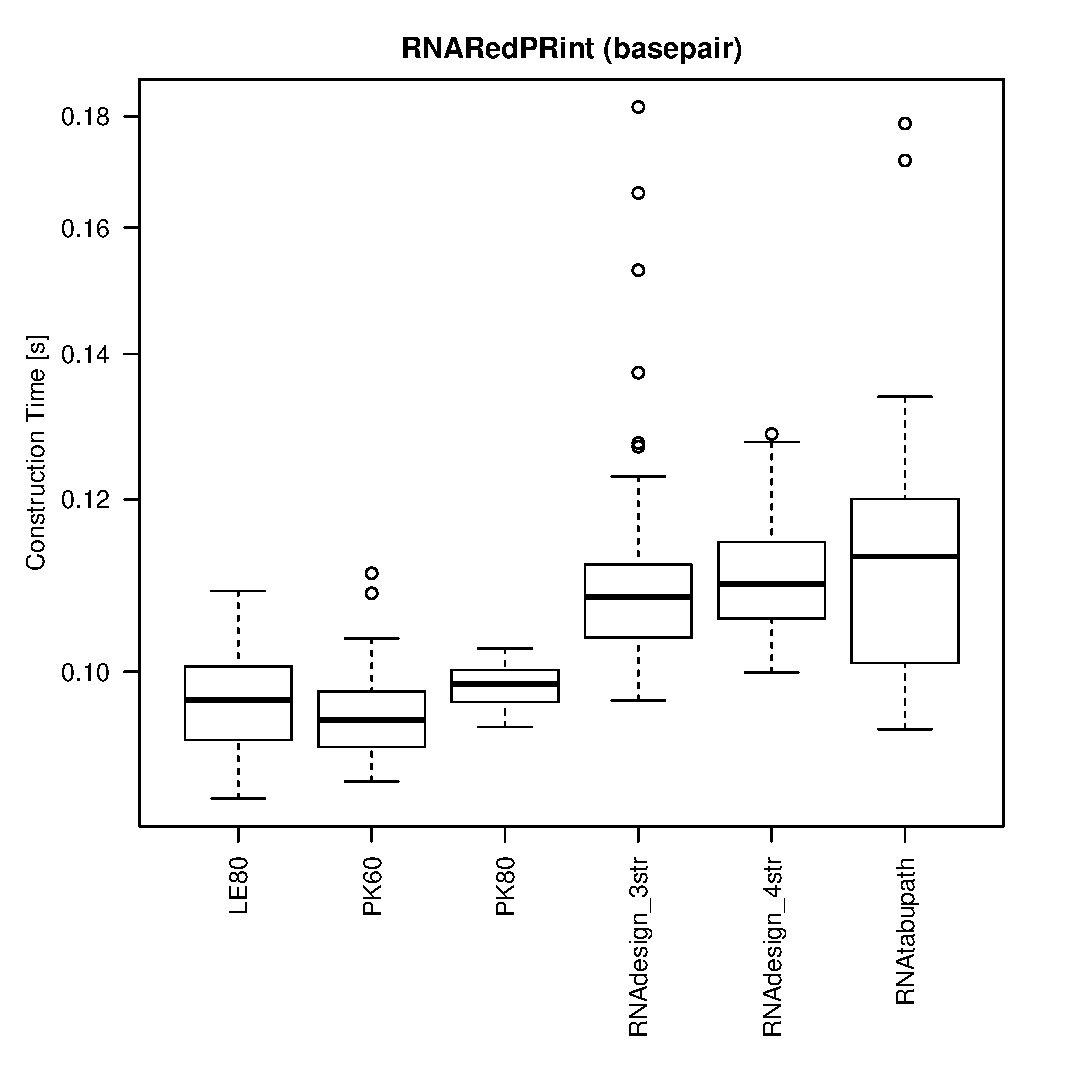
\includegraphics[width=0.45\textwidth]{Figs/RunTimes/construction_time_sets_bp}\quad%
  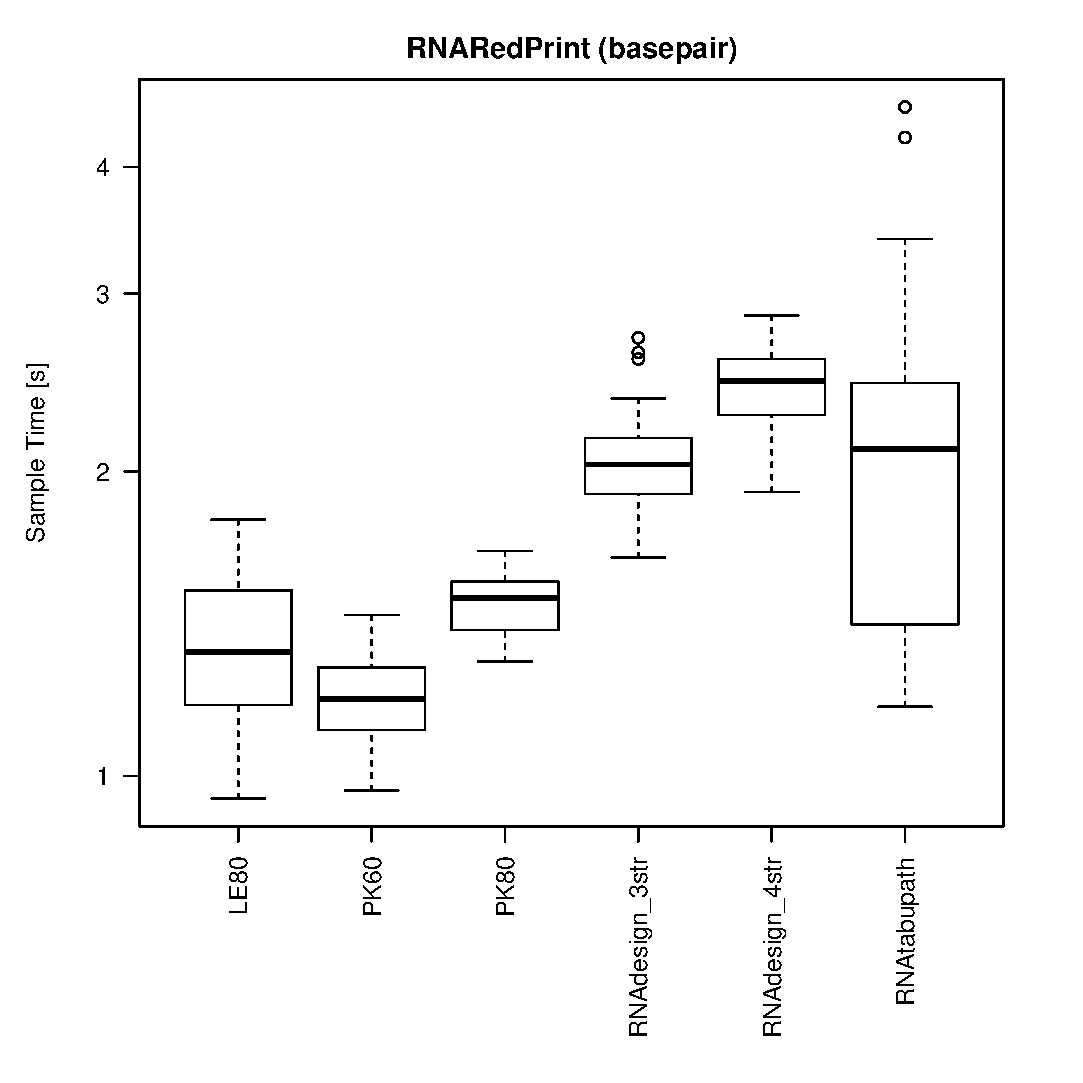
\includegraphics[width=0.45\textwidth]{Figs/RunTimes/sample_time_sets_bp}
  \caption{\todo[inline]{caption Stefan?}}
  \label{fig:run-times-redprint}
\end{figure}
\begin{figure}[tbh]
  \centering
  \includegraphics[width=0.45\textwidth]{Figs/RunTimes/construction_time_sets_rbp}\quad%
  \includegraphics[width=0.45\textwidth]{Figs/RunTimes/sample_time_sets_rbp}
  \caption{\todo[inline]{caption Stefan?}}
  \label{fig:run-times-rbp}
\end{figure}

\end{revision}

\section{Illustrating multi-dimensional Boltzmann sampling for three pseudoknot-free target structures}

    In analogy to Fig.~\ref{fig:energydist-pk} of the main text,
    Fig.~\ref{fig:energydist} illustrates our multi-dimensional sampling
    strategy for three pseudoknot-free target structures (example instance
    from the \texttt{Modena} benchmark). The figure shows Turner energy
    distributions of single structures from sampling with different weight
    parameters, where weights are trained to target specific energies. For
    comparison, the figure shows distributions from uniform and Boltzmann
    sampling at respective homogenous weights $1$ and $e^\beta$.

    Fig.~\ref{fig:gc-content} shows the distributions of the GC content of the samples, while targeting different combinations of energies in this experiment. For completeness, we also report corresponding results for the analogous experiment from the main text. We observe that in addition to the target energies, also the feature $\GCb\%$ is narrowly defined by the multi-dimensional Boltzmann sampling strategy. In comparison, for uniform sampling and Boltzmann sampling at high weight $e^\beta$, where the \GCb\% is not controlled, we obtain much broader distributions. 

\begin{figure}[tb]
      \begin{center}
        %{\sf \bfseries A}\includegraphicstop[width=0.32\textwidth]{Figs/offset2}\hspace{.5cm}
        %{\sf \bfseries B}
        \includegraphicstop[width=0.8\textwidth]{Figs/energy_distribution}
      \end{center}
      \caption{%
        Targeting specific energies using multi-dimensional Boltzmann
        sampling. We show the Turner energy distributions for
        three target structures R1, R2 and R3. By
        targeting the respective free energies $(-40,-40,-20)$ and
        $(-20,-20,-20)$ for the target structures (annotated in red and
        blue, resepectively), we demonstrate the
        effectivity of our adaptive multi-dimensional Boltzmann sampling
        procedure; moreover, for comparison, the distributions for uniform
        (U) and Boltzmann (B) samples---respectively associated with
        homogenous weights $1$ and $e^\beta$.
%    ($\delta=0.05, \delta'=0.1, \gamma=1.1, \psi=20, n=1000$)
  }
  \label{fig:energydist}
\end{figure}

\begin{figure}
  \begin{center}
    {\sf \bfseries A}~\includegraphicstop[width=0.45\textwidth]{Figs/Plots/PKB00211_PKB00239_0_GC_content}
    ~~~~~{\sf \bfseries B}~\includegraphicstop[width=0.45\textwidth]{Figs/Plots/supp_3str_GC_content}
  \end{center}
  \caption{Distribution of the \GCb-content \GCb\% in the experiments of (A) Fig.~\ref{fig:energydist-pk} of the main text and (B) Suppl.~Fig.~\ref{fig:energydist}.}
  \label{fig:gc-content}
\end{figure}

\section{Immediate benefits of positive design for negative design}

Already previous work on RNA Design, e.g. INFO-RNA and Incarnation, observed
that---put briefly---negative design benefits from positive design. Here, more
concretely, we simply \emph{demonstrate} this effect (for small examples), where
we consider \Def{negative design} as  
designing RNA sequences that fold with high probability $Pr(R|S)$ into the
given target structure $R$; and \Def{positive design}, as generating one or
many sequences that have a low energy for $R$.

For each of two small examples, a single-stem and a double-stem structure, we produce a uniform and a weighted Boltzmann
sampling, each of 10000 sequenes. For each sampled sequence $S$, we determine
the Turner energy $E(S,R)$ as well as the
%difference $E_\Delta(S,R)$ of $E(S,R)$ to the ensemble energy $E_{\text{ens}}(S)$ of $S$ 
probability $Pr(R|S)$ of the structure $R$ in the ensemble of sequence $S$ 
(where the energies are calculated in the Turner model using RNAfold). 

Note that low energy $E(S|R)$ is (non-linearly) correlated with high
probability $Pr(S|R)$, the probability to see $S$ in the Boltzmann distribution
of sequences folding into $R$. Recall that the probability $Pr(R|S)$ can be
calculated as $\exp(-E(S,R)/RT)/Z(S)$,
where $Z(S)=\sum_{R'} \exp(-E(S,R')/RT)$.
%
Consequently, Figure~\ref{fig:negforpos} ultimately illustrates the dependencies
between $Pr(S|R)$ and $Pr(R|S)$ for uniform samples and low energy samples
(where those samples can be efficiently generated due to our Boltzmann sampling
strategy). For our examples, we observe (Fig.~\ref{fig:negforpos}) that Boltzmann sampling with weight 500 (green), generates good negative designs 
with substantially higher probability than uniform sampling (blue).

% and high energy difference $E_\Delta(S,R)=E_{\text{ens}}(S)-E(S,R)$, with high probability $\Pr(R|S)$.
% 
% To see the latter, recall that the \Def{ensemble energy $E_{\text{Ens}}(S)$} is defined as
% $$
% E_{\text{ens}}(S) = -RT \ln( Z(S) ),
% $$ 
% based on the partition function $Z(S)=\sum_{R'} \exp(-E(S,R')/RT)$
% such that 
% $$
% E(S,R) - E_{\text{ens}}(S) 
% =
% -RT \ln Pr(R|S),
% $$  
% which can be derived by term transformation 
% \begin{align*}
% -RT \ln P(R|S) &= -RT \ln [ exp(-E(S,R)/RT) / Z(S) ] \\&= -RT \ln (exp(-E(S,R)/RT)) - (-RT\ln Z(S))
% \\&=  E(S,R) - E_{\text{Ens}}(S). 
% \end{align*}

\begin{figure}
\textbf{A}~\includegraphicstop[width=0.48\textwidth]{Figs/Plots/stem_weight1-500_mean}%
\textbf{B}~\includegraphicstop[width=0.48\textwidth]{Figs/Plots/doublestem_weight1-500_mean}%
\caption{Comparison of uniform sampling and Boltzmann sampling with
weight $\pi=500$. We show results for two different small structures: (A) single stem structure (B) double stem structure. For each respective structure $R$, we plot the energies $E(S,R)$ of
10000 sampled sequences against the probabilities $Pr(R|S)$ (in log scale). For illustrating the trend, we show moving averages over windows of $\pm 1$ kcal. Note that while only the energy $E(S,R)$ is directly controlled by Boltzmann sampling, this strongly impacts the common negative design objective $Pr(R|S)$.}
\label{fig:negforpos}
\end{figure}

\section{Parameters for the base pair and the stacking energy model}
\label{appsec:modelparameters}

We trained parameters for two RNA energy models to approximate the
Turner energy model, as implemented in the \Software{ViennaRNA}
package.  In the \Def{base pair model}, the total energy of a sequence $S$
for an RNA structure $R$ is given as sum of base pair energies, where
we consider six types of base pairs distinguishing by the bases $\Ab$-$\Ub$,
$\Cb$-$\Gb$ or $\Gb$-$\Ub$ (symmetrically) and between stacked and non-stacked base
pairs; here, we consider base pairs $(i,j)\in R$ \Def{stacked} iff
$(i+1,j-1)\in R$, otherwise \Def{non-stacked}. In the \Def{stacking model},
our features are defined by the stacks, i.e. pairs $(i,j)$ and
$(i+1,j-1)$ which both occur in $R$; we distinguish 18 types based on
$S_i,S_j,S_{i+1},S_{j-1}$ (i.e. all combinations that allow canonical
base pairs; the configurations $S_i,S_j,S_{i+1},S_{j-1}$ and
$S_{i+1},S_{j-1},S_j,S_i$ are symmetric).

Both models describe the energy assigned to a pair of sequence and
structure in linear dependency of the number of features and their
weights. We can thus train weights for linear predictors of the Turner
energy in both models.

For this purpose, we generated 5000 uniform random RNA sequences of
random lengths between 100 and 200. For each sample, we predict the
minimum free energy and corresponding structure using the ViennaRNA
package; then, we count the distinguished features (i.e., base pair or
stack types). The parameters are estimated fitting linear models
without intercept (\texttt{R} function \texttt{lm}). For both models,
\texttt{R} reports an adjusted R-squared value of 0.99. The resulting
parameters are reported in Tables~\ref{tab:basepairmodel} and
\ref{tab:stackingmodel}.

For validating the trained parameters, we generate a second
independent test set of random RNA sequences in the same
way. Fig.~\ref{fig:training-cor} shows correlation plots for the
trained parameters in the base pair and stacking models for predicting
the Turner energies in the test set with respective correlations of
$0.95$ an $0.94$.

\begin{figure}
  \centering
  A)\includegraphicstop[width=0.4\textwidth,trim=0 0 0 50,clip]{Figs/basepaircor}
  B)\includegraphicstop[width=0.4\textwidth,trim=0 0 0 50,clip]{Figs/stackingcor}
  \caption{Validation of the trained parameters for the A) base pair
    model B) stacking model for predicting energies of the
    independently sampled sequences in the test set. We show
    correlation plots against the Turner energies reported by the
    ViennaRNA package.}
  \label{fig:training-cor}
\end{figure}

\begin{table}[b]
  \centering
  \caption{Trained weights for the base pair energy model.}
  \label{tab:basepairmodel}
  \begin{tabular}{c@{\quad}c@{\quad}c@{\quad}|@{\quad}c@{\quad}c@{\quad}c}
    \multicolumn{3}{c}{non-stacked} & \multicolumn{3}{c}{stacked}\\
    AU      & CG       & GU      & AU       & GC       & GU \\\hline
    1.26630 & -0.09070 & 0.78566 & -0.52309 & -2.10208 & -0.88474
  \end{tabular}
\end{table}

% GC_IN = -0.09070;
% AU_IN = 1.26630;
% GU_IN = 0.78566;
% GC_TERM = -2.10208;
% AU_TERM = -0.52309;
% GU_TERM = -0.88474;

\begin{table}[b]
  \centering
  \caption{Trained weights for the stacking energy model (the rows specify $S_i,S_j$; the columns, $S_{i+1},S_{j-1}$; we do not show the symmetric weights).}
  \label{tab:stackingmodel}
  \begin{tabular}{c@{\quad}|@{\quad}c@{\quad}c@{\quad}c@{\quad}c@{\quad}c@{\quad}c@{\quad}c@{\quad}c}
       & AU & CG & GC & GU & UA & UG \\\hline
    AU &
-0.18826 &
-1.13291 &
-1.09787 &
-0.38606 &
-0.26510 &
-0.62086
    \\
    CG &
-1.11752 &
-2.23740 &
-1.89434 &
-1.22942 &
-1.10548 &
-1.44085
    \\
    GU &
-0.55066 &
-1.26209 &
-1.58478 &
-0.72185 &
-0.49625 &
-0.68876
    \\
  \end{tabular}
\end{table}

\section{Contribution of terms to the MultiDefect score}

\newcommand{\EnsE}{\text{\rm G}} %ensemble energy


Figure~\ref{fig:contribtions-multidefect} breaks down the multi-defect
score of Eq.~$(\ref{eq:blueprintobjective})$, which is used to
evaluate the quality of multi-target designs. Recall that the total
score is composed of the term $\frac{1}{k} \sum_{\ell=1}^{k} (E(S,
R_\ell) - \EnsE(S))$, which evaluates the distances of the energies of
target structures to the minimum free energy (Distance to MFE), and
the term $\frac{1}{2\binom{k}{2}} \sum\limits_{1\leq\ell<j\leq
  k}|E(S,R_\ell) - E(S,R_j)|$, which evaluates the similarity of the
target structure energies of the target structures (Heterogeneity).

\label{appsec:multidefect}
\begin{figure}[h!]
\includegraphics[width=.48\textwidth]{Figs/statistics-Term1}
\includegraphics[width=.48\textwidth]{Figs/statistics-Term2}
\caption{Break-down of average MultiDefect values into their two components.}
\label{fig:contribtions-multidefect}
\end{figure}



\section{Approximate counting and random generation}
In fact, not only is $\#{\sf BIS}$ a reference problem in counting complexity, but it is also a landmark problem with respect to the complexity of approximate counting problems. In this context, it is the representative for a class of $\#{\sf BIS}$-hard problems~\citep{Bulatov2013} that are easier to approximate than $\# {\sf SAT}$, yet are widely believed not to admit any Fully Polynomial-time Randomized Approximation Scheme. Recent results reveal a surprising dichotomy in the behavior of $\#{\sf BIS}$: it admits a Fully Polynomial-Time Approximation Scheme (FPTAS) for graphs of max degree $\le 5$~\citep{Weitz2006}, but is as hard to approximate as the general $\#{\sf BIS}$ problem on graphs of degree $\ge 6$~\citep{Cai2016}. In other words, there is a clear threshold, in term of the max degree, separating (relatively) easy instances from really hard ones.

Additionally, let us note that, from the classic Vizing Theorem, any bipartite graph $G$ having maximum degree $\Delta$ can be decomposed in polynomial time in exactly $\Delta$ matchings. Any such matching can be reinterpreted as a secondary structure, possibly with crossing interactions (\Def{pseudoknots}). These results have two immediate consequences for the pseudoknotted version of the multiple design counting problem.
\begin{corollary}[as follows from~\citep{Weitz2006}]The number of designs compatible with $m\le 5$ pseudoknotted RNA structures can be approximated within any fixed ratio by a deterministic polynomial-time algorithm.
\end{corollary}
\begin{corollary}[as follows from~\citep{Cai2016}]
  As soon as the number of pseudoknotted RNA structures strictly exceeds $5$, \NumDesign is as hard to approximate as {\#{\sf BIS}}.
\end{corollary}

It is worth noting that the $\#{\sf P}$ hardness of \NumDesign does not immediately imply the hardness of generating a valid design uniformly at random, as demonstrated constructively by Jerrum, Valiant and Vazirani~\citep{Jerrum1986}. However, in the same work, the authors establish a strong connection between the complexity of approximate counting and the uniform random generation. Namely, they showed that, for problems associated with self-reducible relations, approximate counting is equally hard as (almost) uniform random generation. We conjecture that the (almost) uniform sampling of sequences from multiple structures with pseudoknots is in fact \#{\sf BIS}-hard as soon as the number of input structures strictly exceeds $5$, as indicated by~\citet{Goldberg2004}, motivating even further our parameterized approach.

\section{Tree decomposition for RNA design instances in practice}
\label{appsec:treedecomp}

For studying the typically expected treewidths and tree decomposition
run times in multi-target design instances, we consider five sets of
multi-target RNA design instances of different complexity. Our first
set consists of the Modena benchmark instances.

In addition, we generated four sets of instances of increasing
complexity. The instances of the sets RF3, RF4, RF5, and RF6, each
respectively specify 3,4,5, and 6 target structures for sequence
length 100.  For each instance (100 instances per set), we generated a
set of $k$ ($k=3,\dots,6$) compatible structures as follows
\begin{itemize}
\item Generate a random sequence of length 100;
\item Compute its minimum free energy structure (ViennaRNA package);
\item Add the new structure to the instances if the resulting base pair dependency graph is bipartite;
\item Repeat until $k$ structures are collected.
\end{itemize}
For each instance, we generated the dependency graphs in the base pair
model and in the stacking model. Then, we performed tree decomposition
(using strategy ``GreedyFillIn'' of LibTW~\citep{Dijk2006}) on each dependency
graph. The obtained treewidths are reported in
Fig.~\ref{fig:td-widths}, while Fig.~\ref{fig:td-times} shows the
corresponding run-times of the tree decomposition.

\revised{
  Finally, for further illustration, we show concrete tree decompositions for a selected instance in the benchmark set RF3 in Figure~\ref{fig:td-example}. Note that this figure is provided solely for illustrational purposes:
  First, it depicts the tree decomposition for a typical, realistic sampling task. Second, it exemplarily illustrates the typical impact of the energy model on the tree decomposition.
  Compared to the tree decomposition based on the stacking model, the tree decomposition for the base pair model is much simpler. This shows in many connected components, which correspond to independently solvable sub-problems, and fewer positions per bag (i.e. smaller tree width), which allows far more efficient evaluation per tree node. 
  Note that the complexity of the tree decomposition ultimately shows the complexity of the dependencies that need to be considered for simultaneous energy evaluation for all target structures. This complexity is substantially increased in the stacking model over the simpler base pair model.
}

\begin{figure}
  %\hspace*{2cm}\textbf{Base pair model}\hspace{4.75cm}\textbf{Stacking model}\\[-28pt]
  \centering\includegraphics[width=0.9\textwidth]{Figs/td-widths}
  \caption{Treewidths for multi-target RNA design instances of
    different complexity. Distributions of treewidths shown as boxplots for the base pair (left) and stacking model (right).}
  \label{fig:td-widths}
\end{figure}

\begin{figure}
  %\hspace*{2cm}\textbf{Base pair model}\hspace{4.75cm}\textbf{Stacking model}\\[-28pt]
  \centering
  \includegraphics[width=0.9\textwidth]{Figs/td-times}
  \caption{Computation time of tree decompositions for
    multi-target RNA design instances of different complexity.
    Distributions of times (in ms/instance) shown as boxplots for the base pair (left) and stacking model (right).}
  \label{fig:td-times}
\end{figure}


\begin{figure}[t!]
  %% the figure shows benchmark_inputs/RNAfold/3str/f3.100.0.inp
  \centering
  \verbatiminput{Figs/f3_100_0.txt}
  \includegraphicstop[width=0.6\textwidth]{Figs/td-example-basepair}%
  \includegraphicstop[width=0.35\textwidth]{Figs/td-example-stacking}
  \caption{Example instance from RF3 (top) with its tree decompositions in the base pair (left) and stacking model (right). The respective treewidths are 2 and 12.}
  \label{fig:td-example}
\end{figure}


\section{Tree decomposition with hyper-dependencies}
\label{appsec:dependency-cliques}

Our implementation relies on external tools for the tree decomposition, which do not directly support tree decomposition of hyper-graphs. Therefore it is not immediately obvious how 
to obtain a suitable tree decomposition, such that even multi-ary contributions are respected and a cluster tree can be generated.

Crucially, one can show that, as long as certain vertices of a graph $G$ from a clique, there exists at least one node in the tree decomposition of $G$ that contains all such vertices.
%
This allows us to generate suitable tree decompositions, which respect the hyper-edges of our dependency graph, by expanding the hyper-edges to cliques, and then calling the tree-decomposer on the resulting (non-hyper-)graph.

%
While the result is certainly part of folklore, we emphasize the importance for the generality of this work and present a brief direct proof for convenience.

\begin{lemma}\label{lem:cliques}
Let $G=(V,E)$ be an undirected graph, and  $(T,\chi)$ be a tree decomposition for $G$. For each clique $C\subseteq V$, there exists a node $u \in T$ such that $C\subseteq\chi(u)$.
\end{lemma}

%\begin{proof}
% \newcommand{\tn}{v_{\rm T}} %% node in tree
% \newcommand{\TransVars}[1]{{\rm tverts}(#1)}
% \newcommand{\Children}[1]{{\rm Children}(#1)}
%  For the sake of simplicity, let us consider $T$ as rooted on an arbitrary node, inducing an orientation, and denote by $\TransVars{\tn}\in V$ the set of vertices found in the node $\tn$ or its descendants, namely
%    $$\TransVars{\tn} = \chi(\tn) \cup \bigcup_{\tn'\in\Children{\tn}} \TransVars{\tn'}.$$
%
%  Now consider (one of) the deepest node(s) $\tn\in T$, such that $C\subseteq\TransVars{\tn}$. We are going to prove that $C\subseteq\chi(\tn)$, using contradiction, by showing that $C\not\subseteq\chi(\tn)$ implies that $T$ is not a tree decomposition.
%
%  Assume that $C\not\subseteq\chi(\tn)$, then there exists a node $v'\notin\chi(\tn)$ whose presence in $\TransVars{\tn}$ stems from its presence in some descendant of $\tn$. Let us denote by $\tn'\neq \tn$ the closest descendant of $\tn$ such that $v'\in\chi(\tn')$. Now, consider a node $v\in C$ such that $v\in \TransVars{\tn'}$ and $v\notin \TransVars{\tn'}$. Such a node always exists, otherwise $\tn'$, and not $\tn$, would be the deepest node such that $C\subseteq \TransVars{\tn'}$. From the definition of the tree decomposition, we know that neither $\tn'$ nor its descendants may contain $v$. On the other hand, none of the parents or siblings of $\tn'$ may contain $v'$. It follows that is no node $\tn''\in T$ whose vertex set $\chi(\tn'')$ includes, at the same time, $v$ and $v'$. Since both $v$ and $v'$ belong to a clique, one has $\{v,v'\}\in E$. The absence of a node in $T$ capturing an edge in $E$ contradicts our initial assumption that $T$ is tree decomposition for $G$.
%
%  We conclude that $\tn$ is such that $C\not\subseteq\chi(\tn)$.
%\end{proof}

\begin{proof}
  \newcommand{\TransVars}[1]{{\rm tverts}(#1)}%
  Root $T$ at an arbitrary tree node $r\in T$, which induces a parent/child relation between tree nodes.
  We say a tree node $u$ \emph{represents} the node $v\in V$ (respectively, the set of nodes $X\subseteq V$) iff $v\in\chi(u)$ ($X\subseteq\chi(u)$).
  Moreover, denote by $\TransVars{u}\subseteq V$ the vertices
  represented by the nodes of the subtree of $u$, i.e.
  $$\TransVars{u} := \chi(u) \cup \bigcup_{\text{children $u'$ of u}} \TransVars{u'}.$$

  Assume there is no node in T that represents $C$.

  Let $u$ denote the node in $T$ with maximal distance to the root $r$,
  such that still $C\subseteq\TransVars{u}$.
  Since there is no single node $u$ that represents $C$, this maximal node is unique, since
  if a node $u$, $C\subseteq\TransVars{u}$, has two subtrees that cover $C$, then $u$ must represent $C$ due to property 2 of Def.~\ref{def:treedecomp}. 

  Let $C'$ be $C-\chi(u)$.
  $C'$ cannot be empty, since otherwise $u$ represents $C$i.
  For exactly one of the children $u'$ of $u$,
  $C'\subseteq\TransVars{u'}$, since otherwise for
  some node $v'\in C'$, the subtree of the nodes representing $v'$ would be disconnected (property 2 of Def.~\ref{def:treedecomp}). Now, pick some $v'\in C'$ and some
  $v''\in C-C'$, which must be represented by $u$ or some child $u''$ of $u$. In both cases, there cannot
  be any node in T that represents the edge $\{v',v''\}\subseteq C$, since $v'$ can only be represented 
  by nodes in the subtree of $u'$. Contradiction.
\end{proof}


This result implies that classic tree decomposition algorithms and, more importantly, implementations can be directly re-used to produce decompositions that capture energy models of arbitrary complexity, functions of arbitrary arity. Indeed, it suffices to add a clique, involving the parameters of the function, and Lemma~\ref{lem:cliques} guarantees that the tree decomposition will feature one node to which the function can be associated.


    \section{Correctness of the FPT partition function algorithm}
    \label{appsec:correctness}

    \begin{theorem}[Correctness of Alg.~\ref{alg:pf}]
      \label{the:pfalgo-correctness}
      As computed by Alg.~\ref{alg:pf} for cluster tree $(T,\chi,\phi)$,
      the messages $\Message{u}{v}$, for all edges $u\to{}v\in T$, yield
      the partition functions of subtree of $u$ for the partial sequences
      $\val\in\partseqs(\separator{u}{v})$, i.e. the messages satisfy
      \begin{equation}
       \evalfor{\Message{u}{v}}{\val} = \sum_{\val'\in\partseqs(\chi(T_r(u))-\separator{u}{v})} \quad
       \prod_{f\in\phi(T_r(u))} \exp(-\evalfor{f}{\substitute{\val'}{\val}}),\label{eq:pfalgo-correct}
     \end{equation}
     where $\chi(T_r(u))$ denotes all $\chi$-assigned positions of nodes in $T_r(u)$;
     respectively $\phi(T_r(u))$; all $\phi$-assigned functions.
    %
    \end{theorem}

    \begin{proof}
      Note that in more concise notation, Alg.~\ref{alg:pf} computes
      messages such that
    \begin{equation}
      \evalfor{\Message{u}{v}}{\val} := \sum_{\val'\in\partseqs(\difference{u}{v})}\quad
      \prod_{f\in \phi(u) } \exp(-\evalfor{f}{\substitute{\val'}{\val}}) \prod_{(w\to{}u) \in T} \evalfor{\Message{w}{u}}{\substitute{\val'}{\val}}.\label{eq:messages}
    \end{equation}

    Proof by induction on $T$. If $u$ is a leaf, $\chi(r) = \chi(T_r(u))$,
    there are no messages sent to $u$, and $\phi(u) = \phi(T_r(u));$ implying
    Eq.~$(\ref{eq:pfalgo-correct}).$
    %
    Otherwise, since the algorithm traverses edges in postorder, $u$ received from its children
    $w_1,\dots,w_q$ the messages $\Message{w_1}{u}, \dots, \Message{w_q}{u}$, which satisfy Eq.~$(\ref{eq:pfalgo-correct})$ (induction hypothesis). Let $\val\in\partseqs(\separator{u}{v})$; then, $\evalfor{\Message{u}{v}}{\val}$ is computed by the algorithm according to Eq.~$(\ref{eq:messages})$. We rewrite as follows
    \begin{align*}
      & \sum_{\val'\in\partseqs(\difference{u}{v})}\quad
        \prod_{f\in \phi(u) } \exp(-\evalfor{f}{\substitute{\val'}{\val}})
        \prod_{(w\to{}u) \in T} \evalfor{\Message{w}{u}}{\substitute{\val'}{\val}}\\
      & = \sum_{\val'\in\partseqs(\chi(u)-\separator{u}{v})}\quad
        \prod_{f\in \phi(u) } \exp(-\evalfor{f}{\substitute{\val'}{\val}})
        \prod_{i=1}^q \evalfor{\Message{w_i}{u}}{\substitute{\val'}{\val}}\\
      & =_{IH}
        \sum_{\val'\in\partseqs(\chi(u)-\separator{u}{v})}\quad
        \prod_{f\in \phi(u) } \exp(-\evalfor{f}{\substitute{\val'}{\val}})
        \prod_{i=1}^q \sum_{\val''\in\partseqs(\chi(T_r(w_i))-\separator{w_i}{u})} \quad
        \prod_{f\in\phi(T_r(w_i))} \exp(-\evalfor{f}{\substitute{\val''}{\substitute{\val'}{\val}}}) \\
    & =_{*}
        \sum_{\val'\in\partseqs(\chi(u)-\separator{u}{v})}\quad
      \sum_{\val''\in\partseqs(\bigcup_{i=1}^q\chi(T_r(w_i))-\separator{w_i}{u})} \quad
      \prod_{f\in \phi(u) } \exp(-\evalfor{f}{\substitute{\val'}{\val}})
      \prod_{f\in\phi(T_r(w_i))} \exp(-\evalfor{f}{\substitute{\val''}{\val'} \cup \val}) \\
      & =_{(**)} \sum_{\val'\in\partseqs(\chi(T_r(u))-\separator{u}{v})}\quad
        \prod_{f\in \phi(T_r(u)) } \exp(-\evalfor{f}{\substitute{\val'}{\val}})\\
    \end{align*}
    To see (*) and (**), we observe:
    \begin{itemize}
    \item The sets $\chi(u)-\separator{u}{v}$ and
      $\chi(T_r(w_i))-\separator{w_i}{u}$ are all disjoint due to
      Def.~\ref{def:treedecomp}, property 2. First, this property implies
      that any shared position between the subtrees of $w_i$ and $w_j$
      must be in $\chi(w_i)$, $\chi(w_j)$ and $\chi(u)$, thus the
      positions of $\chi(T_r(w_i))-\separator{w_i}{u}$ are
      disjoint. Second, if a position $\chi(T_r(w_i))$ occurs in
      $\chi(u)$, it must occur in $\chi(w_i)$ and consequently in $\separator{u}{v}$.
    \item The union of the sets $\chi(u)-\separator{u}{v}$ and
      $\chi(T_r(w_i))-\separator{w_i}{u}$ is $\chi(T_r(u))-\separator{u}{v}).$
    \end{itemize}

    \end{proof}

    \section{General complexity of the partition function computation by cluster tree elimination and generation of samples}
    \label{appsec:algcomplexity}

    \begin{proposition}
      \label{prop:general-complexity}
    Given a cluster tree $(T,\chi,\phi)$, $T=(V,E)$ of the set of contributions $\F{}$ with treewidth $w$ and maximum separator size $s$, computing the partition function by Algorithm~\ref{alg:pf} takes $O((|F|+|V|)\cdot 4^{w+1})$ time and $O(|V| 4^s)$ space (for storing all messages). The sampling step has time complexity of $O((|F|+|V|)\cdot 4^D)$ per sample.
    \end{proposition}

    \begin{proof}[Proposition~\ref{prop:general-complexity}]
    Let $d_u$ denote the degree of node $u$ in $T$, $s_u$ is the size of the separator between
    $u$ and its parent in $T$ rooted at $r$. For each node in the cluster tree, Alg.~\ref{alg:pf} computes one message by combining $(|\phi(u)|+d_u-1)$ functions, each time enumerating $4^{|\chi(u)|}$ combinations; Alg.~\ref{alg:sampling} computes $4^{|\chi{u}|-s_u}$ partition functions each time combining $(|\phi(u)|+d_u-1)$ functions.  $4^{|\chi(u)|}$ is bound by $4^{w+1}$ and $4^{|\chi{u}|-s_u}$ by $4^D$; moreover $\sum_{u\in V} (|\phi(u)|+d_u-1) = |F|+|V|-1$.
    \end{proof}


    \section{Exploiting constraint consistency to reduce the complexity}\label{sec:improvedComplexity}

    While Alg.~\ref{alg:pf} computes messages values for
    \emph{all} possible combinations of nucleotides for the positions
    % in the separator set,
    % yp: for all the positions in a node, right?
    in a node,
    we observe here that many such combinations are \emph{not} required for computing all relevant
    partition functions. In particular, the algorithm can be restricted to
    consider only \Def{valid} combinations, satisfying the (hard)
    constraints induced by valid base pairs.

    The given structures in the RNA design problem impose constraints on
    the sequences for ensuring canonical (aka complementary)
    base pairing. These constraints can be exploited in a particularly
    simple and effective way to reduce the complexity.  As previously
    noted by \citet{Flamm2001}, the base pair complementarity induces a
    bi-partition of each connected component within the base pair
    dependency graph, such that the nucleotides assigned to the two set of
    nodes in the partition are restricted to values in $\{\Ab,\Gb\}$ and
    $\{\Cb,\Ub\}$ respectively. We call a partial sequence \Def{cc-valid},
    iff its determined positions are consistent with such a separation for
    all determined positions of the same connected component.

    % Let $CC=\{cc_1$, $cc_2, \dots\}$ denote the vertex sets of the
    % connected components of the base pair dependency graph. In this graph,
    % let each component have the bi-partition $cc_i=cc^0_i\cup cc^1_i$.

    One can now modify Alg.~\ref{alg:pf}, on a tree decomposition
    $(T,\chi)$, such that the values of messages
    $\Message{u}{v}$ are computed only for cc-valid
    partial sequences $\val\in\partseqs(\separator{u}{v})$. Moreover, the
    loop over $\val'\in\partseqs(\difference{u}{v})$ is restricted, such
    that $\substitute{\val}{\val'}$ are cc-valid. Analogous restrictions are
    then implemented in the sampling algorithm Alg.~\ref{alg:sampling}.

    The correctness of the modified algorithm follows from the same
    induction argument, where the message computation over one node
    evaluates messages from its children only at cc-valid partial
    sequences. The result of this computation is a message, which corresponds
    to the partition function, restricted to cc-valid partial sequences.
    Since invalid sequences have infinite energy, they do not contribute to
    the partition function, and the partition function restricted to cc-valid sequences coincides
    with the initial one.



    This restriction drastically improves the time
    complexity. Indeed, for any given node $v$, the original algorithm sends message for
     $\chi(v):=\substitute{\val}{\val'}$ such that
    $\val\in\partseqs(\separator{u}{v})$ and
    $\val'\in\partseqs(\difference{u}{v})$, while the modified algorithm
    only considers cc-valid assignments for $\chi(v)$. Remark that, in any connected component $cc$,
    assigning some nucleotide to a position reduces cc-valid assignments to (at most)
    two alternatives for each of the $|cc|-1$ remaining positions. It follows that, for a node $v$ featuring positions from $\#cc(v)$ distinct connected components $\{cc_1,cc_2\ldots\}$ in the base pair dependency graph, the number of cc-valid assignments to positions in $\chi(v)$ is exactly
    $$4^{\#cc(v)}\prod_{i=1}^{\#cc(v)} 2^{|cc_i|-1} = 2^{\#cc(v)}\, 2^{|\chi(v)|} \in \Theta(2^{\#cc}\, 2^{w+1}),$$
    for a single node, where $\#cc$ is the total number of connected components in the base pair dependency graph, and $w$ is the tree-width of the tree decomposition $T$. Since the number of nodes in $T$ is in $\Theta(n)$, and the number of atomic energy contributions associated with $k$ structures is in $\mathcal{O}(k\,n)$, then the overall complexity grows like $\Theta(n\, k\, 2^{\#cc}\, 2^{w+1})$.

    %For each connected component having at least a position $i$ in $\chi(v)$,
    %the algorithm considers assigning any possible nucleotide $x\in \Sigma$ to $i$ and restricts
    % the assignment of  for
    %any remaining position $j$ of the same connected component, it restricts the domain of $j$ to base-pairs that are consistent with the parity .
    %
    %
    %Let $c(v)$ be the number of connected components involving positions
    %in $\chi(v)$; then, the first stage enumerates $2^{c(v)}$
    %combinations. For each such combination, the second stage enumerates
    %only $2^{|\chi(v)|}$ partial sequences, since there remain only two
    %possible nucleotide choices for each position. All message values for
    %node $v$ are thus computed in time
    %$\Theta(2^{c(v)+|\chi(v)|})$. Consequently, the total time complexity
    %of the modified algorithm is $$O(nk2^{\hat w}),$$ where $n$ is the RNA
    %length, $k$ is the number of structures, and
    %$\hat w := \max_{v\in T} c(v)+|\chi(v)|$.
    %%
    %From this directly follows the slightly looser complexity
    %bound $$O(nk2^{w+1}2^{c})$$ in terms of treewidth $w$ and the maximum
    %number $c$ of connected components represented in a node of the tree
    %decomposition.  Notably, $\hat w$, as well as $w+1+c$, can not exceed
    %$2(w+1)$, since $c\leq w+1$. Consequently the modified algorithm does
    %never increase the original complexity.

    Finally, we remark that even stronger time savings could be possible
    in practice, since cc-valid partial sequences can still violate
    complementarity constraints, e.g. by assigning C and A to positions in
    different sets of a partition, thus satisfying the bi-partition
    constraints, where the positions base pair directly, rendering the
    partial sequence invalid. Moreover, applications of the sampling
    framework can introduce additional constraints that further reduce
    the number of valid partial subsequences. However, exploiting all such
    constraints, in a complete and general way, would likely cause significant
    implementation overhead, while not significantly improving
    the asymptotic complexity.


    %\section{Exploiting the bipartite nature of base pair dependency
    %  graphs to reduce the complexity}\label{sec:first-improvedComplexity}
    %\textcolor{red}{\textbf{TODO: discuss and merge with/replace by previous Section}}
    %
    %As already noted by \citet{Flamm2001}, the requirement of canonical
    %base pairing induces a bi-partition of each connected component within
    %the base pair dependency graph, such that the nucleotides assigned to
    %the two set of nodes in the partition are restricted to values
    %$\{\Ab,\Gb\}$ and $\{\Cb,\Ub\}$ respectively.
    %%
    %It follows that, within each connected component of the base pair
    %dependency graph, the assignment of any position drastically restricts
    %the domain of the remaining positions, \emph{i.e.} they may now be
    %assigned to only 2 out of the original 4 nucleotides.
    %\newcommand{\Parity}[1]{p_{#1}} To exploit this property, and further
    %reduce the exponential factor of the complexity, we introduce the
    %notion of \Def{parity} of a vertex/position, whereby vertices of
    %\Def{even} (resp. \Def{odd}) polarities may only be assigned values in
    %$\{\Ab,\Gb\}$ (resp. $\{\Cb,\Ub\}$). Neighbors of an odd vertex must
    %be even and vice versa, so the choice of a parity for any single
    %vertex caracterizes the parity of all vertices in a bipartite
    %connected subgraph.
    %
    %Let $CC=\{cc_1,cc_2,\ldots\}$ denote the connected components of the base pair dependency graph, we consider a modified version of the cluster tree, obtained by:
    %\begin{enumerate}
    %\item Electing, in each connected component $cc_i$, the first position $v_i^\star$ from the component encountered from the root in a pre-order traversal of the cluster tree;\label{step:election}
    %\item Introducing new variables $\mathcal{P}=\{\Parity{1},\ldots,\Parity{|CC|}\}$, representing the parity of elected vertices;
    %\item Adding, to each node $x$ in the tree decomposition, the parity variables of connected components that are represented in the node, \emph{i.e.} such that at least one of the positions in the connected component is in $\chi(x)$; \label{step:addparities}
    %\item Introducing, in the tree decomposition, a chain of intermediate nodes to fix cases where more than a single (parity) variable is introduced between a parent and its child.\label{step:intermediates}
    %\end{enumerate}
    %Note that, since connected components correspond to connected subtrees in the tree decomposition, then adding those variables preserves the properties of a tree decomposition. Also, each node in the former cluster tree introduces at most one new variable compared to its parent, so the elected node is uniquely defined by the rule stated in Step~\ref{step:election}. Finally, we note that the parity of a variable $v\in cc_i$ is entirely characterized by the parity $\Parity{i}$ of $v_i^\star$, and the parity of the distance between $v$ and $v_i^\star$ in the base pair dependency graph. Namely, the parity of $v$ is $\Parity{i}$ if the distance between $v$ and $v^{\star}_i$ is even, and opposite to $\Parity{i}$ if odd. It follows that, thanks to the new variables introduced in Step~\ref{step:addparities}, the domain of each of the original variables can be reduced to two alternatives instead of the original four.
    %
    %The computation of Alg.~\ref{alg:pf} on the new cluster tree, considering reduced assignments for position variables and additional odd/even assignments for parity variables, has complexity in $\mathcal{O}(n\,k\,2^{w+1}\,2^{c})$, where $n$ is the RNA length, $k$ is the number of structures, $w$ is the tree-width of the unmodified cluster tree, and $c$ is the maximum number of connected components represented in a node. It should be noted that $c\le \min(|CC|,w+1)$, so that the new complexity cannot be larger than the one stated in Th.~\ref{th:complexities}. Also, note that the number of nodes introduced by Step~\ref{step:intermediates} is bounded by $|CC|$, so that the introduction of these intermediate nodes does not impact the worst-case complexity. For the same reason, the complexity of the stochastic backtrack remains unchanged.


\section{Monotonicity of the partial derivatives within weight calibration}
\label{sec:weight_derivatives}
%
In weighted distributions, one witnesses a fairly predictable impact of the variation of any weight $\pi_\ell$ over the expected value $\mathbb{E}(E_\ell\mid \pmb{\pi})$, $\pmb{\pi}:= (\pi_1\cdots\pi_k)$, of the free energy $E_\ell$ of structure $\ell$.  Let us  first remind the probability of a sequence $S$ in the weighted distribution
\begin{align*}
  \mathcal{B}_{\pmb{\pi}}(S) &= \prod_{i=1}^{k} \pi_i^{-E_i(S)}, &
  \partfun{\pmb{\pi}}&=\sum_{S'}\mathcal{B}_{\pmb{\pi}}(S') &
    \text{and}& &
  \mathbb{P}(S\mid \pmb{\pi}) &= \frac{\mathcal{B}_{\pmb{\pi}}(S)}{\partfun{\pmb{\pi}}}.
  \end{align*}

Remind also the definition of the expectation of $E_\ell(S)$, for $S$ a Boltzmann-distributed sequence:
$$\mathbb{E}(E_\ell\mid \pmb{\pi}) = \sum_S E_\ell(S)\cdot \mathbb{P}(S\mid \pmb{\pi}).$$

We first remark that the partial derivative of $\mathcal{B}$ yields
\begin{align*}
  \frac{\partial \mathcal{B}_{\pmb{\pi}}(S)}{\partial \pi_\ell} = -E_\ell(S)\cdot \pi_\ell^{-E_\ell(S)-1}\prod_{\substack{i=1\\i\neq \ell}}^{k} \pi_i^{-E_i(S)} = \frac{-E_\ell(S)}{\pi_\ell}\cdot\mathcal{B}_{\pmb{\pi}}(S) = -E_\ell(S)\cdot \mathbb{P}(S\mid \pmb{\pi})\cdot \frac{\partfun{\pmb{\pi}}}{\pi_\ell }
\end{align*}
while the partial derivative of $\mathcal{Z}$ gives
\begin{align*}
  \frac{\partial \partfun{\pmb{\pi}}(S)}{\partial \pi_\ell} = \sum_{S'} -E_\ell(S')\cdot \mathbb{P}(S'\mid \pmb{\pi})\cdot \frac{\partfun{\pmb{\pi}}}{\pi_\ell }= -\mathbb{E}(E_\ell\mid \pmb{\pi})\cdot \frac{\partfun{\pmb{\pi}}}{\pi_\ell}.
\end{align*}
From these expressions, we conclude that
\begin{align*}
  \frac{\partial \mathbb{E}(E_\ell\mid \pmb{\pi})}{\partial \pi_\ell} &= \sum_S E_\ell(S)\cdot\frac{\partial \mathbb{P}(S\mid \pmb{\pi})}{\partial \pi_\ell}\\
  %
  & = \sum_S E_\ell(S)\left(\frac{\frac{\partial \mathcal{B}_{\pmb{\pi}}(S)}{\partial \pi_\ell}}{\mathcal{Z}_{\pmb{\pi}}} - \frac{\frac{\partial \mathcal{Z}_{\pmb{\pi}}}{\partial \pi_\ell}\cdot\mathcal{B}_{\pmb{\pi}}(S)}{\mathcal{Z}_{\pmb{\pi}}^2}\right)\\
  %
  & = \sum_S E_\ell(S)\left(\frac{-E_\ell(S)\cdot \mathbb{P}(S\mid \pmb{\pi})\cdot \frac{\mathcal{Z}_{\pmb{\pi}}}{\pi_\ell }}{\mathcal{Z}_{\pmb{\pi}}} + \frac{\mathbb{E}(E_\ell\mid \pmb{\pi})\cdot \frac{\mathcal{Z}_{\pmb{\pi}}}{\pi_\ell}\cdot\mathcal{B}_{\pmb{\pi}}(S)}{\mathcal{Z}_{\pmb{\pi}}^2}\right)\\
  %
  & = \sum_S - \frac{E_\ell(S)^2\cdot\mathbb{P}(S\mid \pmb{\pi})}{\pi_\ell} + \frac{\mathbb{E}(E_\ell\mid \pmb{\pi})}{\pi_\ell}\sum_S E_\ell(S)\cdot \mathbb{P}(S\mid \pmb{\pi})\\
  & = -\frac{\mathbb{E}(E_\ell^2\mid \pmb{\pi}) - \mathbb{E}(E_\ell\mid \pmb{\pi})^2}{\pi_\ell}
\end{align*}
In the numerator of the above expression, one recognizes the variance of the distribution of $E_\ell$.
Remark that a variance is always non-negative and, in our case, also strictly positive for $\pmb{\pi}$, $\pi_\ell>0$, as soon as there exist at least two distinct sequences $S$ and $S'$ such that $E_\ell(S)\neq E_\ell(S')$.
Moreover, weights are always positive so the partial derivative in $\pi_\ell$ is always positive. Ultimately, it is always possible to increase (resp. decrease) the expected free energy of a structure by simply decreasing (resp. increasing) its weight, supporting our weight optimization procedure.



\section{Detailed results of MultiDefect analysis}\label{sec:validity}
N/A values correspond to data that could not be obtained by the time of this submission for two main reasons: In the case of the initial sampling (left columns), they correspond to instances which, in conjunction with an expressive energy model, resulted in very high tree-width, leading to unreasonable memory requirements incompatible with our available computing resources; The case of missing values after optimization  (right columns), they indicate situations where the initial optimization took too long ($\approx$ 1 day) and was killed.
\subsection{RNAtabupath (2 structures)}
{
\begin{longtable}{@{}cr@{\hspace{1em}}r@{\hspace{1em}}r@{\hspace{1em}}r@{\hspace{1em}}r@{\hspace{2em}}r@{\hspace{1em}}r@{\hspace{1em}}r@{\hspace{1em}}r@{\hspace{1em}}r@{}}
\toprule
&\multicolumn{2}{@{}l@{}}{Boltzmann}&\multicolumn{2}{@{}l@{}}{Uniform}&&\multicolumn{2}{@{}l@{}}{\begin{minipage}[b]{1.8cm}Boltzmann\\Optimized\end{minipage}}&\multicolumn{2}{@{}l@{}}{\begin{minipage}[b]{1.8cm}Uniform\\Optimized\end{minipage}}&\ \\
Name&Mean&StdDev&Mean&StdDev&$\Delta$&Mean&StdDev&Mean&StdDev&$\Delta_{\text{opt}}$\\
\toprule
alpha\_operon&17.15&4.06&25.86&5.97&8.70&2.13&0.83&2.36&0.88&0.23\\
amv&14.34&2.87&27.26&5.65&12.92&3.75&0.90&4.27&1.08&0.52\\
attenuator&10.80&3.03&21.44&4.77&10.64&1.37&0.53&1.81&0.80&0.44\\
dsrA&11.81&2.58&18.23&4.62&6.42&3.75&0.94&3.80&0.95&0.06\\
hdv&22.00&4.81&35.48&6.68&13.47&3.64&1.14&4.57&1.48&0.92\\
hiv&41.07&7.02&73.00&9.40&31.92&17.07&3.26&30.06&5.34&12.99\\
ms2&13.36&3.72&19.79&4.55&6.43&2.36&0.79&2.66&0.97&0.30\\
rb1&18.40&4.48&37.38&7.14&18.98&2.63&0.92&3.82&1.31&1.19\\
rb2&16.59&4.10&25.17&5.85&8.58&2.81&0.84&3.07&0.97&0.26\\
rb3&22.43&4.57&41.18&7.09&18.75&2.77&0.82&5.05&1.52&2.27\\
rb4&26.11&4.32&47.89&6.80&21.77&7.00&1.15&11.80&1.82&4.80\\
rb5&30.77&5.47&54.24&7.76&23.48&6.01&1.96&9.22&2.78&3.21\\
ribD&49.88&7.09&81.27&9.07&31.39&20.35&3.27&30.75&4.33&10.39\\
s15&10.93&2.94&18.37&4.53&7.44&1.95&0.67&2.12&0.77&0.16\\
sbox&24.93&4.63&50.03&8.04&25.10&6.28&1.56&9.08&2.28&2.80\\
spliced&9.65&2.96&17.60&4.39&7.95&2.15&0.46&2.41&0.59&0.26\\
sv11&20.95&4.63&36.83&6.91&15.88&3.04&0.88&4.20&1.12&1.17\\
thim&29.23&5.43&48.32&6.95&19.09&8.58&1.86&12.12&2.54&3.54\\
\midrule
Mean&21.69&4.37&37.74&6.45&16.05&5.42&1.27&7.95&1.75&2.53\\
\bottomrule
\end{longtable}}
\subsection{RNADesign (3 structures)}
{
\begin{longtable}{@{}cr@{\hspace{1em}}r@{\hspace{1em}}r@{\hspace{1em}}r@{\hspace{1em}}r@{\hspace{2em}}r@{\hspace{1em}}r@{\hspace{1em}}r@{\hspace{1em}}r@{\hspace{1em}}r@{}}
\toprule
&\multicolumn{2}{@{}l@{}}{Boltzmann}&\multicolumn{2}{@{}l@{}}{Uniform}&&\multicolumn{2}{@{}l@{}}{\begin{minipage}[b]{1.8cm}Boltzmann\\Optimized\end{minipage}}&\multicolumn{2}{@{}l@{}}{\begin{minipage}[b]{1.8cm}Uniform\\Optimized\end{minipage}}&\ \\
Name&Mean&StdDev&Mean&StdDev&$\Delta$&Mean&StdDev&Mean&StdDev&$\Delta_{\text{opt}}$\\
\toprule
sq100&20.73&5.02&31.78&5.46&11.05&5.81&1.53&8.33&1.92&2.53\\
sq10&19.73&5.27&26.62&5.59&6.89&3.50&0.81&3.88&0.94&0.38\\
sq11&19.46&4.73&27.76&5.69&8.30&2.81&0.77&3.31&0.89&0.49\\
sq12&17.09&3.57&22.62&4.98&5.53&2.70&0.65&2.79&0.68&0.09\\
sq13&18.55&3.96&29.95&5.56&11.40&10.24&2.18&16.63&3.13&6.39\\
sq14&21.52&4.25&37.82&5.55&16.31&7.25&1.63&9.90&2.10&2.65\\
sq15&21.93&3.77&36.32&5.13&14.39&11.15&1.75&15.49&2.34&4.33\\
sq16&15.86&4.23&27.70&5.58&11.84&2.51&0.69&2.96&0.94&0.45\\
sq17&20.66&3.69&33.62&5.33&12.97&5.83&1.08&7.36&1.49&1.52\\
sq18&19.70&3.86&35.26&5.13&15.57&5.83&1.41&7.97&2.00&2.14\\
sq19&14.78&3.37&28.64&5.34&13.86&3.84&0.77&4.66&1.04&0.82\\
sq1&14.75&3.75&21.89&5.48&7.14&2.02&0.65&2.20&0.69&0.18\\
sq20&17.41&3.81&27.90&4.93&10.48&3.93&1.04&5.18&1.48&1.24\\
sq21&21.66&4.03&36.27&5.16&14.60&8.28&1.82&11.41&2.40&3.12\\
sq22&17.69&4.13&31.57&5.45&13.89&5.66&1.51&10.02&2.50&4.36\\
sq23&19.35&3.61&32.38&5.40&13.03&12.05&1.85&18.69&3.18&6.65\\
sq24&17.96&4.03&27.92&5.30&9.96&3.59&0.93&4.25&1.10&0.66\\
sq25&17.65&5.10&26.65&6.11&9.00&1.35&0.34&1.45&0.40&0.10\\
sq26&17.64&4.51&24.46&5.64&6.82&3.11&0.62&3.38&0.68&0.27\\
sq27&18.08&3.57&28.51&5.30&10.43&7.55&1.49&10.96&2.38&3.41\\
sq28&14.90&3.66&29.35&5.99&14.46&2.32&0.49&2.66&0.62&0.34\\
sq29&17.65&3.69&26.95&5.08&9.30&4.44&0.98&5.22&1.21&0.78\\
sq2&22.38&4.17&37.25&5.15&14.87&10.34&1.71&14.32&2.35&3.99\\
sq30&19.14&4.08&31.75&5.54&12.62&6.06&1.61&8.99&2.19&2.93\\
sq31&19.94&3.83&31.92&5.20&11.98&5.12&1.19&6.34&1.55&1.22\\
sq32&22.06&3.99&31.65&5.23&9.59&5.24&1.29&6.84&1.76&1.60\\
sq33&15.21&4.28&22.75&5.52&7.54&1.78&0.43&2.08&0.63&0.30\\
sq34&25.01&4.14&37.46&5.03&12.46&12.46&1.84&18.73&2.57&6.27\\
sq35&19.12&4.11&32.72&5.35&13.61&5.90&1.25&7.96&1.82&2.06\\
sq36&12.72&2.81&26.76&5.39&14.04&3.19&0.77&3.61&0.94&0.41\\
sq37&18.72&3.83&32.44&5.62&13.72&3.24&0.90&4.21&1.25&0.98\\
sq38&14.73&3.61&29.02&5.29&14.29&2.79&0.86&3.70&1.22&0.91\\
sq39&22.75&3.96&33.06&4.98&10.30&9.20&1.76&11.87&2.33&2.67\\
sq3&20.34&4.02&36.86&5.60&16.52&4.69&1.19&6.30&1.72&1.61\\
sq40&19.52&4.33&31.76&5.41&12.24&4.05&0.94&4.96&1.19&0.91\\
sq41&14.44&3.48&27.85&5.57&13.41&3.33&0.71&3.91&0.88&0.58\\
sq42&18.68&3.89&35.20&5.55&16.51&5.32&1.24&6.96&1.56&1.64\\
sq43&17.32&3.94&31.63&5.38&14.31&3.53&0.89&4.27&1.15&0.74\\
sq44&19.38&3.66&31.75&5.09&12.37&5.52&1.29&7.26&1.60&1.74\\
sq45&18.49&4.74&27.40&5.53&8.90&2.54&0.67&2.84&0.74&0.30\\
sq46&17.97&3.84&28.83&5.09&10.86&4.45&0.90&5.41&1.20&0.96\\
sq47&15.22&3.86&28.23&5.82&13.01&3.02&0.78&3.45&0.85&0.43\\
sq48&18.89&4.14&36.27&5.78&17.38&4.69&1.08&6.71&1.67&2.02\\
sq49&20.19&4.73&27.24&5.39&7.05&3.15&0.76&3.66&0.95&0.51\\
sq4&19.32&4.73&29.25&5.34&9.93&2.36&0.79&3.24&1.15&0.88\\
sq50&16.92&3.83&28.43&5.35&11.51&3.15&0.73&3.54&0.86&0.38\\
sq51&22.17&4.07&36.07&5.20&13.90&11.56&1.79&16.57&2.88&5.01\\
sq52&19.33&3.94&31.04&5.20&11.71&11.04&2.21&16.25&3.04&5.21\\
sq53&13.65&3.69&24.48&5.46&10.83&1.65&0.39&1.88&0.53&0.23\\
sq54&18.25&3.67&33.99&5.57&15.74&8.15&1.57&12.35&2.59&4.19\\
sq55&22.12&4.75&30.11&5.21&8.00&4.59&0.82&5.43&1.13&0.83\\
sq56&17.85&3.90&31.69&5.46&13.84&4.22&0.75&4.84&0.93&0.62\\
sq57&16.39&4.07&28.48&5.45&12.08&1.96&0.58&2.28&0.71&0.32\\
sq58&12.73&2.86&32.97&5.80&20.24&3.77&0.82&4.89&1.22&1.11\\
sq59&20.45&4.54&33.02&5.57&12.57&6.05&1.50&8.34&2.08&2.29\\
sq5&9.90&2.70&17.94&4.93&8.04&1.29&0.33&1.41&0.39&0.12\\
sq60&22.73&4.85&36.86&5.46&14.13&6.90&1.62&11.07&2.33&4.17\\
sq61&14.34&3.75&30.82&6.03&16.48&3.07&0.76&3.83&1.01&0.76\\
sq62&21.12&5.04&35.27&5.35&14.15&9.76&1.67&16.93&2.79&7.17\\
sq63&13.38&3.56&27.20&5.63&13.82&1.58&0.36&1.85&0.53&0.27\\
sq64&19.19&3.90&34.88&5.24&15.69&6.10&1.53&9.45&2.29&3.35\\
sq65&19.39&4.58&27.51&5.15&8.12&13.95&2.94&19.40&3.61&5.45\\
sq66&18.14&3.71&30.79&5.12&12.65&6.93&1.42&10.05&2.03&3.12\\
sq67&20.62&3.40&37.06&5.18&16.44&16.11&1.97&27.21&3.40&11.10\\
sq68&23.09&4.33&33.33&5.08&10.24&6.99&1.55&9.23&1.94&2.24\\
sq69&18.76&3.63&35.06&5.21&16.29&10.77&1.94&18.38&3.00&7.61\\
sq6&20.48&3.75&38.48&5.48&18.00&5.55&1.32&8.63&2.04&3.08\\
sq70&13.52&3.25&31.06&5.52&17.54&2.59&0.80&3.80&1.17&1.21\\
sq71&20.04&4.04&32.71&5.39&12.67&5.57&1.06&6.61&1.30&1.04\\
sq72&14.96&3.15&24.48&4.94&9.51&2.02&0.57&2.49&0.84&0.47\\
sq73&14.97&3.75&28.44&5.56&13.47&2.34&0.69&3.10&1.04&0.75\\
sq74&17.77&4.06&30.13&5.30&12.36&4.12&0.79&5.03&1.04&0.91\\
sq75&19.63&4.00&31.19&5.19&11.56&5.63&1.26&7.52&1.70&1.89\\
sq76&19.91&3.93&32.44&5.12&12.53&9.12&1.92&13.89&2.39&4.78\\
sq77&18.70&3.45&34.83&5.21&16.12&6.01&1.25&8.61&1.75&2.61\\
sq78&18.29&3.50&32.94&6.01&14.66&5.39&1.12&7.07&1.51&1.68\\
sq79&21.66&4.74&30.73&5.47&9.07&13.10&2.89&17.86&3.45&4.75\\
sq7&20.44&3.92&32.95&5.41&12.52&5.51&1.70&6.68&1.90&1.17\\
sq80&15.57&3.93&28.29&5.30&12.71&1.85&0.53&2.41&0.88&0.56\\
sq81&21.44&4.58&29.92&5.44&8.48&3.74&0.95&4.67&1.33&0.93\\
sq82&8.94&2.38&19.89&5.36&10.94&1.39&0.21&1.47&0.28&0.09\\
sq83&14.12&3.47&28.92&5.45&14.80&2.77&0.76&3.52&1.01&0.75\\
sq84&15.63&3.94&24.12&5.26&8.49&2.54&0.47&2.85&0.65&0.31\\
sq85&15.54&3.43&26.09&5.18&10.55&2.19&0.62&2.70&0.82&0.51\\
sq86&21.77&5.09&34.21&5.77&12.43&4.66&1.21&5.92&1.51&1.26\\
sq87&16.55&3.87&32.65&5.81&16.10&3.50&0.62&4.14&0.86&0.64\\
sq88&20.10&5.08&33.45&5.86&13.34&2.50&0.72&3.17&0.99&0.68\\
sq89&14.74&4.28&26.15&5.59&11.41&1.79&0.50&2.01&0.62&0.23\\
sq8&15.80&4.14&30.34&6.02&14.55&2.85&0.79&3.85&1.15&1.00\\
sq90&15.30&3.88&29.83&5.80&14.53&2.10&0.64&2.90&1.06&0.79\\
sq91&17.38&3.99&27.19&5.08&9.81&3.69&1.11&4.48&1.31&0.79\\
sq92&19.15&3.54&33.07&5.34&13.91&4.77&1.11&6.83&1.78&2.06\\
sq93&19.54&4.22&29.17&5.65&9.63&3.29&0.80&3.86&1.03&0.57\\
sq94&14.79&3.26&27.05&5.43&12.26&3.98&0.77&4.66&0.98&0.68\\
sq95&17.58&3.67&33.42&5.38&15.84&12.86&2.20&22.76&3.84&9.90\\
sq96&15.44&3.87&31.62&5.68&16.18&2.69&0.67&3.52&1.02&0.83\\
sq97&18.38&3.98&29.22&5.03&10.83&4.31&1.13&5.32&1.42&1.01\\
sq98&18.83&4.59&29.30&5.42&10.47&2.78&0.73&3.59&0.97&0.80\\
sq99&19.61&4.14&30.95&5.28&11.34&3.94&0.98&4.89&1.33&0.95\\
sq9&17.05&4.26&26.15&5.72&9.11&1.66&0.44&1.79&0.55&0.13\\
\midrule
Mean&18.10&3.98&30.49&5.41&12.39&5.10&1.10&7.04&1.52&1.94\\
\bottomrule
\end{longtable}}
\subsection{RNADesign (4 structures)}
{
\begin{longtable}{@{}cr@{\hspace{1em}}r@{\hspace{1em}}r@{\hspace{1em}}r@{\hspace{1em}}r@{\hspace{2em}}r@{\hspace{1em}}r@{\hspace{1em}}r@{\hspace{1em}}r@{\hspace{1em}}r@{}}
\toprule
&\multicolumn{2}{@{}l@{}}{Boltzmann}&\multicolumn{2}{@{}l@{}}{Uniform}&&\multicolumn{2}{@{}l@{}}{\begin{minipage}[b]{1.8cm}Boltzmann\\Optimized\end{minipage}}&\multicolumn{2}{@{}l@{}}{\begin{minipage}[b]{1.8cm}Uniform\\Optimized\end{minipage}}&\ \\
Name&Mean&StdDev&Mean&StdDev&$\Delta$&Mean&StdDev&Mean&StdDev&$\Delta_{\text{opt}}$\\
\toprule
sq100&21.70&4.41&33.19&4.93&11.49&12.32&2.52&17.14&3.10&4.82\\
sq10&20.66&5.16&27.00&5.24&6.34&6.63&1.91&8.02&2.05&1.39\\
sq11&22.23&4.23&30.73&5.31&8.50&6.18&1.30&7.70&1.70&1.52\\
sq12&18.30&3.55&23.38&4.93&5.08&3.78&0.57&3.94&0.64&0.17\\
sq13&21.01&3.57&31.66&4.93&10.65&15.61&1.75&21.61&2.69&6.00\\
sq14&22.46&3.09&39.77&5.28&17.31&17.59&2.28&25.04&3.21&7.45\\
sq15&22.66&3.72&36.31&5.01&13.65&17.42&2.41&26.80&3.34&9.38\\
sq16&18.22&4.12&28.54&5.33&10.32&3.29&0.76&3.78&0.90&0.50\\
sq17&23.04&4.01&35.87&5.28&12.82&12.63&2.37&18.43&2.86&5.79\\
sq18&21.20&3.49&35.78&5.39&14.57&8.24&1.53&10.75&2.02&2.51\\
sq19&15.36&2.73&32.12&4.95&16.76&13.30&1.67&23.64&3.41&10.34\\
sq1&15.14&3.83&22.32&5.28&7.18&2.53&0.56&2.66&0.56&0.13\\
sq20&16.75&3.09&29.25&4.74&12.50&9.37&1.60&13.40&2.41&4.03\\
sq21&23.98&3.72&38.18&5.14&14.20&16.47&2.08&23.31&3.16&6.83\\
sq22&20.38&3.81&32.90&5.12&12.53&8.58&1.42&12.39&2.03&3.81\\
sq23&18.39&3.36&32.82&5.34&14.43&12.09&1.81&19.58&3.26&7.50\\
sq24&20.05&4.10&29.72&5.29&9.67&5.45&1.10&7.28&1.68&1.84\\
sq25&21.48&5.35&28.83&5.78&7.35&2.85&0.63&3.30&0.77&0.45\\
sq26&20.83&4.63&27.39&5.25&6.56&4.17&0.76&4.80&0.96&0.63\\
sq27&17.14&3.48&29.41&5.24&12.27&7.56&1.42&11.67&2.34&4.12\\
sq28&23.50&4.48&33.84&6.07&10.35&5.61&1.10&6.69&1.39&1.07\\
sq29&18.14&3.65&27.22&4.85&9.08&5.47&0.88&6.26&1.17&0.78\\
sq2&22.16&3.44&36.10&4.90&13.94&&&24.62&2.30&24.62\\
sq30&19.40&3.76&32.40&4.95&13.00&8.77&1.58&12.39&2.19&3.62\\
sq31&24.97&3.80&32.68&5.19&7.72&8.71&1.28&13.05&2.15&4.34\\
sq32&19.62&3.76&31.03&4.97&11.41&5.47&1.23&7.57&1.71&2.10\\
sq33&19.51&4.25&27.65&5.12&8.14&4.30&0.96&5.37&1.16&1.07\\
sq34&25.15&3.97&37.58&4.90&12.43&14.29&1.86&20.62&2.68&6.33\\
sq35&21.87&3.93&35.50&5.73&13.63&9.63&1.52&13.80&2.31&4.17\\
sq36&11.65&2.59&26.29&5.48&14.64&3.30&0.63&3.86&0.90&0.56\\
sq37&25.80&4.48&36.19&4.90&10.39&15.78&2.11&23.46&2.85&7.68\\
sq38&17.74&3.43&32.11&5.14&14.37&4.95&0.98&6.20&1.38&1.25\\
sq39&21.54&3.83&32.74&5.21&11.20&9.77&1.72&13.10&2.29&3.33\\
sq3&20.19&4.06&39.87&5.23&19.68&14.54&2.18&26.21&3.32&11.67\\
sq40&18.68&4.18&33.41&5.62&14.73&4.29&0.95&5.49&1.30&1.20\\
sq41&15.86&3.46&30.06&5.30&14.19&5.52&0.95&6.59&1.17&1.08\\
sq42&21.79&3.25&38.72&5.11&16.93&14.45&2.03&23.27&3.45&8.82\\
sq43&23.21&3.99&33.89&5.33&10.68&7.16&1.30&9.08&1.76&1.92\\
sq44&21.65&3.59&33.47&4.99&11.83&8.02&1.47&10.91&1.97&2.89\\
sq45&19.01&4.79&27.79&5.58&8.78&3.48&0.66&3.81&0.83&0.33\\
sq46&20.08&3.60&30.69&4.89&10.61&7.76&1.30&9.95&1.73&2.18\\
sq47&17.29&3.73&29.94&5.26&12.65&4.47&1.00&5.23&1.20&0.76\\
sq48&28.78&4.03&38.24&5.57&9.46&16.85&1.71&25.59&3.19&8.73\\
sq49&19.19&4.75&27.33&5.42&8.14&3.14&0.76&3.65&0.86&0.52\\
sq4&19.71&4.46&29.44&5.30&9.73&3.37&0.89&4.26&1.18&0.89\\
sq50&19.36&4.11&30.60&5.49&11.24&4.98&0.81&5.73&0.99&0.75\\
sq51&24.16&2.87&38.68&5.02&14.52&20.73&1.51&28.05&2.50&7.32\\
sq52&21.40&3.37&33.80&5.43&12.40&16.23&2.28&25.12&3.70&8.90\\
sq53&15.81&3.50&28.75&5.32&12.94&4.20&0.99&6.20&1.53&2.00\\
sq54&18.16&3.45&35.10&4.86&16.93&15.41&2.16&26.23&3.39&10.82\\
sq55&22.47&4.43&31.94&5.15&9.47&10.91&2.50&15.20&2.91&4.28\\
sq56&21.11&4.12&35.25&5.93&14.15&12.20&2.06&18.65&2.91&6.44\\
sq57&18.94&3.91&30.86&5.51&11.92&3.69&0.74&4.50&0.90&0.81\\
sq58&19.68&2.97&35.80&5.41&16.12&9.76&1.44&16.74&2.69&6.98\\
sq59&20.35&3.75&33.08&5.20&12.73&17.54&3.02&24.34&3.91&6.81\\
sq5&11.60&2.54&19.61&5.12&8.01&1.90&0.38&2.13&0.49&0.23\\
sq60&21.97&4.37&38.39&5.44&16.42&17.46&2.56&29.58&3.88&12.12\\
sq61&19.07&3.46&34.14&5.24&15.07&7.04&1.32&10.28&1.97&3.24\\
sq62&25.71&5.09&34.50&4.88&8.79&12.06&1.87&17.32&2.60&5.26\\
sq63&17.21&3.45&30.71&5.37&13.50&5.47&1.33&7.39&1.83&1.92\\
sq64&19.89&3.52&35.51&4.96&15.62&13.87&2.03&22.12&3.10&8.24\\
sq65&18.69&4.06&29.18&5.34&10.50&12.71&2.30&17.66&2.97&4.96\\
sq66&17.50&3.40&30.59&5.16&13.09&8.67&1.59&13.61&2.42&4.94\\
sq67&22.63&4.21&36.73&5.06&14.10&17.08&2.27&26.85&3.33&9.77\\
sq68&24.93&4.36&35.00&5.13&10.07&12.42&1.87&17.96&2.39&5.54\\
sq69&22.48&3.16&36.07&4.91&13.59&19.69&1.64&24.53&2.08&4.84\\
sq6&22.32&3.77&40.27&5.41&17.95&6.16&1.36&9.46&2.08&3.29\\
sq70&16.97&4.07&31.84&5.51&14.87&3.60&0.84&5.09&1.32&1.49\\
sq71&19.34&4.07&31.81&5.24&12.47&5.14&0.95&6.26&1.20&1.12\\
sq72&16.60&3.01&29.22&4.92&12.62&6.11&1.17&7.67&1.57&1.55\\
sq73&18.64&3.44&30.86&5.16&12.23&12.22&2.59&21.15&4.05&8.93\\
sq74&17.24&3.88&31.19&5.47&13.95&12.62&3.37&21.49&4.11&8.87\\
sq75&18.44&3.60&31.25&5.19&12.82&7.25&1.35&11.19&2.21&3.94\\
sq76&20.76&3.38&33.74&4.94&12.98&16.76&2.27&25.18&3.38&8.42\\
sq77&21.92&3.29&35.83&5.26&13.91&10.39&1.64&13.96&2.25&3.58\\
sq78&23.60&3.17&36.23&5.47&12.64&19.10&2.58&26.07&3.61&6.96\\
sq79&24.77&4.43&32.49&5.23&7.71&17.83&2.85&23.78&3.64&5.95\\
sq7&19.94&3.54&32.78&5.29&12.84&5.35&1.64&6.59&1.89&1.24\\
sq80&18.63&3.88&29.75&5.27&11.12&2.84&0.64&3.64&1.01&0.80\\
sq81&23.57&3.63&36.02&5.24&12.45&17.61&2.27&25.76&3.17&8.15\\
sq82&13.21&3.25&25.45&5.00&12.24&3.01&0.68&4.06&1.00&1.05\\
sq83&14.37&3.21&31.96&5.41&17.59&3.85&0.89&5.55&1.31&1.70\\
sq84&19.05&3.89&29.35&5.00&10.31&5.20&0.99&6.38&1.32&1.18\\
sq85&17.32&3.91&30.80&5.43&13.48&10.64&2.01&17.53&2.93&6.89\\
sq86&25.19&4.04&36.79&5.66&11.60&8.98&1.94&14.14&2.62&5.16\\
sq87&16.91&3.89&32.84&5.34&15.94&4.86&0.75&6.08&1.18&1.22\\
sq88&22.92&4.99&35.87&5.65&12.95&5.21&0.97&6.58&1.30&1.37\\
sq89&17.52&3.91&29.24&5.45&11.72&4.12&0.87&4.83&1.11&0.71\\
sq8&25.56&4.49&33.42&5.21&7.86&9.60&1.55&12.55&2.05&2.94\\
sq90&18.67&3.62&33.21&5.33&14.54&5.41&1.01&7.26&1.62&1.85\\
sq91&18.00&3.83&26.82&4.85&8.82&8.10&1.80&11.08&2.41&2.98\\
sq92&24.32&3.52&37.62&4.84&13.30&20.06&2.17&29.08&3.47&9.02\\
sq93&22.63&4.66&33.40&5.25&10.77&11.48&2.12&16.37&3.00&4.88\\
sq94&14.71&3.25&28.06&5.39&13.35&3.76&0.76&4.51&0.97&0.75\\
sq95&23.77&4.11&36.93&5.11&13.17&16.41&2.12&23.98&2.67&7.57\\
sq96&17.20&3.70&33.01&5.46&15.81&5.90&1.14&8.09&1.71&2.19\\
sq97&19.78&3.85&30.01&5.09&10.23&6.14&1.24&7.45&1.60&1.31\\
sq98&21.39&4.33&31.13&5.16&9.73&4.74&0.78&5.67&1.03&0.94\\
sq99&20.33&4.39&29.97&5.07&9.64&4.03&1.07&4.95&1.28&0.92\\
sq9&18.86&4.22&29.51&5.22&10.65&3.94&0.90&5.06&1.35&1.11\\
\midrule
Mean&20.15&3.83&32.32&5.23&12.17&9.17&1.51&13.25&2.13&4.17\\
\bottomrule
\end{longtable}}
\subsection{Pseudoknots (PK60)}
{
\begin{longtable}{@{}cr@{\hspace{1em}}r@{\hspace{1em}}r@{\hspace{1em}}r@{\hspace{1em}}r@{\hspace{2em}}r@{\hspace{1em}}r@{\hspace{1em}}r@{\hspace{1em}}r@{\hspace{1em}}r@{}}
\toprule
&\multicolumn{2}{@{}l@{}}{Boltzmann}&\multicolumn{2}{@{}l@{}}{Uniform}&&\multicolumn{2}{@{}l@{}}{\begin{minipage}[b]{1.8cm}Boltzmann\\Optimized\end{minipage}}&\multicolumn{2}{@{}l@{}}{\begin{minipage}[b]{1.8cm}Uniform\\Optimized\end{minipage}}&\ \\
Name&Mean&StdDev&Mean&StdDev&$\Delta$&Mean&StdDev&Mean&StdDev&$\Delta_{\text{opt}}$\\
\toprule
no10&8.77&3.14&17.74&4.46&8.96&1.13&1.19&4.39&1.88&3.26\\
no11&9.40&3.11&16.91&4.07&7.51&2.12&1.12&4.20&1.83&2.08\\
no12&10.81&3.09&21.95&4.54&11.14&3.61&1.05&6.74&2.01&3.13\\
no13&12.33&2.73&21.72&4.06&9.40&4.71&1.26&7.94&2.23&3.23\\
no14&9.51&3.00&19.13&4.27&9.62&2.23&0.98&5.23&1.76&3.00\\
no15&11.62&2.96&18.90&4.16&7.28&4.07&1.15&6.40&1.72&2.33\\
no16&13.14&3.09&19.67&4.19&6.53&4.03&1.17&6.36&1.77&2.33\\
no17&16.39&3.20&21.04&4.29&4.65&6.39&1.23&7.82&1.61&1.42\\
no18&11.41&3.37&18.95&4.41&7.55&1.80&1.75&4.86&2.11&3.06\\
no19&11.06&3.35&20.90&4.27&9.84&2.03&1.49&6.40&2.19&4.37\\
no1&11.88&2.85&22.33&4.39&10.45&3.78&0.99&7.58&1.93&3.80\\
no20&14.55&2.99&19.17&3.97&4.63&5.21&1.16&7.08&1.64&1.87\\
no21&15.73&3.62&22.73&4.36&7.01&6.25&1.36&8.29&1.83&2.04\\
no22&10.23&2.97&15.62&4.03&5.39&1.51&0.97&3.86&1.68&2.35\\
no23&11.64&2.11&16.35&4.40&4.71&3.85&1.04&4.86&1.35&1.01\\
no24&13.13&2.68&18.57&4.17&5.45&3.79&1.28&5.83&1.72&2.04\\
no25&5.91&2.46&16.02&4.18&10.11&0.26&0.72&2.95&1.59&2.69\\
no26&10.57&3.06&19.60&4.19&9.03&3.43&1.04&6.45&1.84&3.02\\
no27&14.49&2.46&23.32&4.62&8.83&4.62&1.33&7.81&2.02&3.19\\
no28&12.29&3.13&24.00&4.50&11.72&3.96&1.53&7.91&2.63&3.95\\
no29&15.59&3.67&21.57&4.49&5.98&4.17&1.49&6.74&2.00&2.57\\
no2&14.21&3.16&24.61&4.36&10.40&6.21&1.46&10.51&2.19&4.30\\
no30&11.76&3.11&17.60&4.02&5.84&4.33&0.81&5.45&1.11&1.11\\
no31&17.81&3.07&25.41&4.05&7.60&8.59&1.48&11.76&2.14&3.17\\
no32&14.07&2.58&18.81&4.05&4.74&5.76&1.13&6.69&1.52&0.93\\
no33&13.37&2.93&21.19&4.08&7.82&3.48&1.55&7.62&2.16&4.14\\
no34&13.19&3.42&18.98&3.93&5.79&4.87&1.67&6.92&1.70&2.05\\
no35&10.85&3.37&14.92&4.25&4.06&1.19&0.87&3.15&1.54&1.96\\
no36&8.33&1.73&17.80&4.16&9.47&2.95&0.97&5.55&1.47&2.59\\
no37&15.99&3.20&26.35&4.39&10.36&7.89&1.65&11.31&2.52&3.41\\
no38&12.51&3.47&19.50&4.08&6.99&2.83&1.32&6.14&1.84&3.32\\
no39&7.57&2.57&14.40&3.94&6.84&1.58&0.93&3.27&1.43&1.69\\
no3&9.65&2.56&18.95&4.43&9.31&1.98&1.04&4.07&1.68&2.08\\
no40&9.44&2.81&17.18&4.10&7.74&3.09&1.06&5.21&1.65&2.12\\
no41&14.91&3.53&20.91&4.48&6.00&4.99&1.08&7.49&1.70&2.50\\
no42&12.05&3.52&22.44&4.50&10.39&3.44&1.44&7.42&2.43&3.99\\
no43&14.07&3.64&21.99&4.15&7.92&5.00&1.23&8.29&1.82&3.29\\
no44&14.09&3.27&22.28&4.14&8.19&4.89&1.60&8.39&2.40&3.50\\
no45&12.67&3.46&22.20&4.33&9.53&3.72&1.36&7.52&2.17&3.80\\
no46&11.25&3.09&19.16&4.32&7.92&3.77&1.27&5.51&1.73&1.74\\
no47&14.02&3.71&23.03&4.43&9.01&5.23&1.63&8.38&2.18&3.16\\
no48&13.03&2.67&24.04&4.48&11.01&5.13&1.30&8.14&2.00&3.01\\
no49&11.49&3.77&18.51&4.19&7.02&2.76&1.20&5.04&1.90&2.28\\
no4&10.74&3.02&18.92&4.21&8.18&3.25&1.37&6.14&1.87&2.89\\
no50&12.19&3.13&19.72&4.34&7.53&4.10&1.34&5.87&1.83&1.77\\
no5&15.97&3.08&19.10&3.96&3.13&7.55&0.92&8.47&1.27&0.92\\
no6&11.44&2.95&16.57&4.42&5.13&2.95&1.12&4.43&1.40&1.48\\
no7&6.50&2.68&12.99&4.20&6.49&0.65&0.78&2.00&1.37&1.35\\
no8&15.01&2.70&20.66&3.93&5.65&6.69&1.18&8.40&1.70&1.70\\
no9&7.45&2.96&15.95&4.18&8.50&0.32&1.09&3.58&1.88&3.26\\
\midrule
Mean&12.12&3.04&19.81&4.24&7.69&3.84&1.23&6.45&1.84&2.58\\
\bottomrule
\end{longtable}}
\subsection{Pseudoknots (PK80)}
{
\begin{longtable}{@{}cr@{\hspace{1em}}r@{\hspace{1em}}r@{\hspace{1em}}r@{\hspace{1em}}r@{\hspace{2em}}r@{\hspace{1em}}r@{\hspace{1em}}r@{\hspace{1em}}r@{\hspace{1em}}r@{}}
\toprule
&\multicolumn{2}{@{}l@{}}{Boltzmann}&\multicolumn{2}{@{}l@{}}{Uniform}&&\multicolumn{2}{@{}l@{}}{\begin{minipage}[b]{1.8cm}Boltzmann\\Optimized\end{minipage}}&\multicolumn{2}{@{}l@{}}{\begin{minipage}[b]{1.8cm}Uniform\\Optimized\end{minipage}}&\ \\
Name&Mean&StdDev&Mean&StdDev&$\Delta$&Mean&StdDev&Mean&StdDev&$\Delta_{\text{opt}}$\\
\toprule
no10&8.42&3.78&18.34&4.91&9.91&-0.53&1.83&3.19&2.18&3.73\\
no11&13.68&3.79&24.67&4.97&10.99&2.89&1.42&7.45&2.66&4.56\\
no12&15.00&3.06&22.26&4.84&7.26&4.23&1.48&6.91&2.13&2.69\\
no13&13.62&4.21&23.33&4.91&9.71&2.80&1.52&7.42&2.39&4.62\\
no14&11.77&4.14&24.61&5.11&12.84&1.16&1.71&7.11&2.62&5.95\\
no15&8.83&3.02&21.68&5.11&12.85&1.90&1.36&5.75&2.17&3.85\\
no16&16.73&3.84&25.45&4.93&8.72&4.85&1.71&8.75&2.46&3.90\\
no17&13.29&3.55&26.27&4.85&12.98&3.11&1.63&10.39&2.72&7.28\\
no18&15.42&3.88&25.61&4.75&10.19&4.07&2.03&7.90&2.57&3.83\\
no19&13.75&4.06&19.53&4.83&5.78&1.97&1.30&4.11&2.07&2.14\\
no1&17.32&4.56&25.64&5.06&8.32&4.59&1.58&8.62&2.43&4.03\\
no20&19.67&3.80&25.88&5.06&6.21&5.44&1.76&8.44&2.32&3.00\\
no21&19.96&3.54&31.00&4.98&11.05&9.09&1.76&14.15&2.57&5.06\\
no22&13.65&3.20&24.94&4.91&11.29&4.68&1.25&8.80&2.20&4.12\\
no23&12.98&3.15&20.28&4.68&7.29&4.54&1.42&6.15&1.81&1.61\\
no24&15.50&3.66&25.89&5.02&10.39&4.63&2.04&9.13&2.57&4.50\\
no25&14.84&4.18&27.83&5.01&12.99&4.02&2.19&9.80&2.75&5.78\\
no26&15.75&3.59&27.66&5.01&11.91&7.02&1.95&13.46&2.62&6.44\\
no27&19.33&3.55&31.95&4.84&12.63&9.79&2.04&15.87&2.86&6.08\\
no28&11.89&3.44&25.54&5.17&13.66&3.25&1.40&8.40&2.51&5.14\\
no29&17.60&4.42&23.52&5.13&5.92&4.03&1.52&6.91&2.17&2.87\\
no2&9.86&2.54&18.04&4.64&8.18&2.55&0.99&4.01&1.46&1.46\\
no30&12.37&3.49&23.07&4.83&10.70&3.17&1.74&7.65&2.41&4.49\\
no3&15.15&3.77&22.49&5.04&7.34&3.54&1.41&7.08&2.21&3.54\\
no4&11.10&2.79&24.80&4.95&13.70&2.01&1.46&8.97&2.64&6.96\\
no5&13.47&3.73&24.27&5.13&10.80&3.23&1.24&8.07&2.34&4.83\\
no6&4.89&3.44&17.34&4.71&12.45&-2.94&1.61&3.26&2.28&6.20\\
no7&12.98&2.54&25.77&4.84&12.79&4.66&1.43&9.68&2.09&5.03\\
no8&14.01&4.16&24.12&4.96&10.11&4.12&1.44&8.11&2.09&3.99\\
no9&11.37&3.97&19.71&4.71&8.33&1.24&1.40&4.04&2.16&2.80\\
\midrule
Mean&13.81&3.63&24.05&4.93&10.24&3.64&1.59&7.99&2.35&4.35\\
\bottomrule
\end{longtable}}
\subsection{LE80}
{
\begin{longtable}{@{}cr@{\hspace{1em}}r@{\hspace{1em}}r@{\hspace{1em}}r@{\hspace{1em}}r@{\hspace{2em}}r@{\hspace{1em}}r@{\hspace{1em}}r@{\hspace{1em}}r@{\hspace{1em}}r@{}}
\toprule
&\multicolumn{2}{@{}l@{}}{Boltzmann}&\multicolumn{2}{@{}l@{}}{Uniform}&&\multicolumn{2}{@{}l@{}}{\begin{minipage}[b]{1.8cm}Boltzmann\\Optimized\end{minipage}}&\multicolumn{2}{@{}l@{}}{\begin{minipage}[b]{1.8cm}Uniform\\Optimized\end{minipage}}&\ \\
Name&Mean&StdDev&Mean&StdDev&$\Delta$&Mean&StdDev&Mean&StdDev&$\Delta_{\text{opt}}$\\
\toprule
PKB00002\_PKB00004\_0&8.78&2.66&14.95&3.72&6.16&2.24&0.91&4.09&1.31&1.84\\
PKB00005\_PKB00015\_0&9.69&3.10&12.97&3.27&3.28&2.91&0.92&4.13&1.06&1.23\\
PKB00008\_PKB00031\_0&10.62&2.40&12.56&3.33&1.94&2.91&0.78&4.11&0.99&1.19\\
PKB00010\_PKB00066\_0&7.07&2.06&12.79&3.32&5.73&2.64&0.80&3.63&1.07&1.00\\
PKB00012\_PKB00268\_0&8.77&2.59&12.54&3.38&3.77&2.77&0.90&3.69&1.10&0.92\\
PKB00030\_PKB00045\_0&6.31&1.82&12.63&3.44&6.32&1.79&0.73&3.39&1.10&1.59\\
PKB00047\_PKB00069\_0&15.24&2.54&19.86&3.99&4.62&6.69&1.26&7.73&1.48&1.05\\
PKB00048\_PKB00265\_0&10.02&3.36&18.64&4.04&8.62&3.77&1.09&8.21&1.74&4.44\\
PKB00050\_PKB00128\_0&11.11&3.77&16.42&4.42&5.30&1.90&1.06&3.72&1.46&1.82\\
PKB00052\_PKB00107\_0&6.72&2.72&16.17&4.45&9.45&1.43&1.07&3.82&1.43&2.40\\
PKB00057\_PKB00072\_0&12.13&2.89&19.82&4.42&7.68&5.34&1.24&7.70&1.72&2.37\\
PKB00068\_PKB00129\_0&15.42&3.03&23.78&4.67&8.36&7.01&0.98&8.84&1.49&1.83\\
PKB00070\_PKB00244\_0&9.22&2.84&18.45&4.09&9.23&2.49&1.35&5.57&1.78&3.07\\
PKB00078\_PKB00106\_0&4.45&2.08&18.46&4.51&14.01&0.12&1.00&4.62&1.85&4.50\\
PKB00080\_PKB00132\_0&8.13&2.10&13.01&3.47&4.89&2.20&0.79&3.40&1.17&1.20\\
PKB00088\_PKB00127\_0&7.00&3.06&19.26&4.94&12.26&0.89&1.03&4.53&1.82&3.64\\
PKB00098\_PKB00232\_0&13.16&3.07&21.53&4.33&8.37&5.38&1.20&8.00&1.64&2.62\\
PKB00131\_PKB00205\_0&11.86&2.78&22.53&4.12&10.67&5.17&1.21&7.67&1.79&2.50\\
PKB00139\_PKB00141\_0&12.53&2.91&19.13&4.33&6.61&4.14&1.00&6.46&1.58&2.31\\
PKB00142\_PKB00231\_0&14.46&3.53&19.98&4.91&5.52&4.51&1.50&6.29&1.87&1.79\\
PKB00143\_PKB00233\_0&9.67&3.05&17.78&4.36&8.11&2.96&1.12&5.47&1.66&2.52\\
PKB00148\_PKB00218\_0&12.06&3.00&22.54&4.75&10.48&5.54&1.38&8.79&2.07&3.26\\
PKB00175\_PKB00259\_0&9.21&2.09&17.94&4.14&8.73&3.99&0.87&6.22&1.42&2.24\\
PKB00179\_PKB00280\_0&16.60&2.06&23.05&5.63&6.45&3.32&1.43&4.88&1.73&1.55\\
PKB00180\_PKB00212\_0&13.09&2.12&21.19&4.75&8.09&5.23&1.45&7.23&1.91&2.01\\
PKB00190\_PKB00266\_0&6.13&2.85&12.98&3.52&6.85&0.21&0.97&2.20&1.34&1.99\\
PKB00207\_PKB00213\_0&6.60&3.00&12.03&3.39&5.43&1.14&0.83&2.56&1.08&1.42\\
PKB00211\_PKB00239\_0&12.92&3.59&22.54&4.81&9.61&4.82&1.44&8.91&2.10&4.09\\
PKB00222\_PKB00305\_0&16.14&2.91&26.40&5.73&10.26&6.64&1.66&9.07&2.12&2.43\\
PKB00224\_PKB00281\_0&10.61&3.09&14.72&3.58&4.11&3.01&1.05&4.34&1.28&1.33\\
PKB00230\_PKB00273\_0&7.91&2.41&15.08&3.80&7.16&3.89&1.31&6.56&1.82&2.67\\
PKB00248\_PKB00257\_0&9.72&3.12&18.37&4.20&8.64&6.44&1.31&11.39&2.71&4.95\\
PKB00263\_PKB00270\_0&12.00&2.17&18.83&4.19&6.83&4.53&1.09&6.34&1.58&1.81\\
PKB00269\_PKB00272\_0&12.93&3.37&16.19&3.78&3.26&4.10&1.20&6.19&1.75&2.09\\
\midrule
Mean&10.54&2.77&17.80&4.17&7.26&3.59&1.11&5.88&1.59&2.28\\
\bottomrule
\end{longtable}}



\bibliographystyle{vancouver}
%\bibliographystyle{achemnat}
%\bibliographystyle{plainnat}
%\bibliographystyle{abbrv}
%\bibliographystyle{bioinformatics}
%
%\bibliographystyle{plain}
%
\bibliography{biblio}


\end{document}
